\subsection{Citizen empowerment}

\subsubsection{Smart communities}
Though most often referred to on the city level, smart communities leverage information and communication technologies (ICT) (networks) and various sources of data (sensors) to address and improve the functional needs of its population (actuators), engaging its ``users'' to develop citizen-centered interventions and responding to their changing needs\cite{Williams2016,Roche2012, Afzalan2017}. %{\color{orange}“A smart community may be one of any size or significance, geographically separate or part of some larger urban unit, that employs the IOT to: improve aspects of its operations or other factors within or outside its boundaries that are important to its economic vitality, safety, environmental footprint, quality fo life or other factors deemed significant; respond to the community’s changing needs rapidly and efficiently; engage the community and enable informed understanding of, and where applicable consent to, what it is doing; collaborate with other communities as needed or desired.”\cite{Williams2016}};{\color{orange}“A smart city is roughly described as a platform or a system of systems, essentially based on three components: Sensors, Networks and Engagement (actuators).” \cite{Roche2012}.}; {\color{orange}“Information and Communication Technologies (ICTs) have given rise to the ideal that cities will become increasingly smart, connected, responsive, and citizen-centric”.}\cite{Afzalan2017}\\
In fact, {“[a]n active and engaged citizen is indeed the main driving force of a `smart city'''\cite{Oliveira2021}}. Though smart cities also address economic vitality and environmental impact in addition to social well-being, empowered communities increasingly expect the ability to influence their environments, such by affecting goverments planning procedures and services\cite{Williams2016}. %-{\color{orange}Smart community: “Communities can be large or small, and they may or may not be ac enter of some noteworthy aspect of human activity; they may be separated from other communities or they may be aggregated into a conurbation of some kind. But any community of any size or significance can be ‘smart’. Communities should also define the services of interest to them, within their territorial boundary or outside it, as required.”\cite{Williams2016}}; -{\color{orange}“there are dimensions of smart which the community pursues.”\cite{Williams2016}}\\
Beyond efficiency, citizens require safer, more enjoyable living experiences in all aspects of their lives. Governments may accommodate the public interest\cite{Afzalan2017}  %-{\color{orange}“Planning and decision making is not all about efficiency, but also about responding to the public interest and community needs.”}\cite{Afzalan2017}\\
by incorporating four dimensions (intelligence, digital, open, and live, referring to its social and informational infrastrucutres, open governance, and continuity of adaptation, respectively) of  smart communities\cite{Oliveira2021}. %- {\color{orange}“There are four dimensions in which a smart city primarily operates, names: intelligent city (its social infrastructure), the digital city (informational infrastructure), the open city (open governance) and the live city (a continuous adaptive urban living fabric) \cite{Oliveira2021}}.\\
The identification and monitoring of community dynamics requires ``sensing life'' though open dialogues with constituents as well as internet of things (IOT: the integration of networked hardware sensors to monitor and/or interact with their surroundings) technology\cite{Roche2012}. %{\color{orange}“Making a city smarter is neither only a technological infrastructure issue, nor a managerial one. It is also and essentially providing citizens a better and safer way of living in urban areas, in teh places where they live, work, have fun, consume… Therefore, sensing life in those places is a major stake to understand new city dynamics and then to design better living urban environments.”} \cite{Roche2012}\\
This sensing infrastructure leverages various sources of data to determine the state of various subsystems and support interventions for improvement. %- {\color{purple}Leverages various sources of data to determine the state of various subsystems and support interventions for improvement.}  \\
Ideally, it may identify potential opportunities for improvement but is more commonly leveraged in application focused scenarios, in which a ``search, evaluate, and process'' method is employed in response to a particular challenge\cite{Jiang2020}. %{\color{orange}“In the big data era, the typical scenario does not start from data but from application. THe research procedure is shifting to a new scenario - ‘search, evaluate, and process’ -, that is, identifying the applications, discovering all data related, adn running a processing model for knowledge generating.”\cite{Jiang2020}}\\

The information age itself is a source of both challenges and potential solutions. 
Since the turn of the century, all facets of urban life and the structures that support them have transitioned towards the digital and informational, .% -{\color{orange}“DUring the last two ecads, urban structures have become more digital and information-based, and there has been a decisive change in the living environment of citizens.”\cite{Rivera2020}}\\
A community as "a system of systems"\cite{Roche2012} %{\color{orange}“A smart city is roughly described as a platform or a system of systems, essentially based on three components: Sensors, Networks and Engagement (actuators).” \cite{Roche2012}.}
has an internal structure\cite{MasseyD1991}, %{\color{orange}“‘Communities’ too have internal structures.”}\cite{MasseyD1991}\\
with corresponding spheres of influence of its nodes within and outside of these.  
As quickly as informational technology (IT) tools provide new means of characterising the immediate, physical geographic area of a community node, it also supports the digital transmission of ideas and participation to remote parties via direct communication platforms as well as the more public arenas of social media. In short: "the geography of social relations is changing"\cite{MasseyD1991}, %-{\color{orange}“the geography of social relations is changing. In many cases such relations are increasingly stretched out over space. Economic, political and cultural social relations, each full of power and with internal structures of domination and subordination, stretched out over the platen at every different level, from the household to the local area to the international.”}\cite{MasseyD1991}\\
with digital connections offering  "unique opportunities to identify and understand information dissemination mechanisms and patterns of activity in both the geographical and social dimensions, allowing us to optimize reponses to specific events"\cite{Oliveira2021}.%- {\color{orange}“As the popularity of social media is growing exponentially we are presented with unique opportunities to identify and understand information dissemination mechanisms and patterns of activity in both the geographical and social dimensions, allowing us to optimize responses to specific events," \cite{Oliveira2021} }
Data in general is already highly regarded as a key comodity for developing an economy\cite{Lupi2017}, % -{\color{orange}“Data is now recognized as one of the founding pillars of our economy, and the notion that the world grows exponentially richer in data every day is already yesterday’s news.”\cite{Lupi2017}}\\
To harness the value of this ever-expanding resource, community operations should accommodate methods for capture, exploring, and sharing this data, spatial or otherwise, and its processed results\cite{Roche2012}.% - {\color{orange}``the need of an enabling geospatial information platform to facilitate data discovery and access in order to support smart cities’ operations.” \cite{Roche2012}.}\\
Beyond operational efficiency, the information products and services have the potential to stimulate new creative uses that facilitate the economic, social, and environmental well-being of the participants of the community\cite{Rajabifard2009}. %-{\color{orange}“The creation of economic wealth, social stability and environmental protection in line with MDGs can be achieved through the development of products and services based on spatial information collected by all levels of government. These goals and objectives can be facilitated through the development of a spatially enabled government and society, where location and spatial information are regarded as common goods made available to citizens and businesses to encourage creativity and product development.” MDG: Millennium Development Goals}\cite{Rajabifard2009}\\
Just as the context of a community -- its culture, history, environment, access to technology, demographics, etc. -- can vary tremendously across time and space, so too should its interventions\cite{Afzalan2017}. %-{\color{orange} “The issue of context-sensitivity may require more attention from planning organizations that try to choose new technologies. Cities are overwhelmed with the availability of new communication technologies and the opportunities that the technologies offer. This issue also exacerbates with the social pressure they receive from citizens who expect the implementation of smarter governance systems.”}\cite{Afzalan2017}\\
Members of such knoweldge societies\cite{Rivera2020} %-{\color{orange} Smart city and knowledge society.\cite{Rivera2020}}\\
, investigators and entrepreneurs or anyone with with access to technology, are better equiped to address local psychographics ("the prevailing interests of people in an area"\cite{Chiappinelli2020} %-{\color{orange}Psychographics: “the prevailing interests of people in the area.”}\cite{Chiappinelli2020}\\
in nontraditional or niche applications\cite{McQueenBaker2019}.  %-{\color{orange}“Increased accessibility of technology pushes researchers to consider how these tools might be used in critical scholarship in nontraditional ways.”\cite{McQueenBaker2019}}\\
Such opportunities can even unburden institutions with the responsibility of managing, processing, and transforming data into relevant services, and instead allow the community itself to develop novel applications for public resource that can be adapted into operations when mature.

%%%%%%%%%%%%%%%%%%%
%- Unlike traditional polling, which attempts to gauge the public pulse on a variety of political and social issues, social media platforms and forums allow the unsoliscited, unformatted presentation of personal perspectives and permit the public evolution of dialogue around these ideas. {\color{purple}News reporting as a more official or pre-aggregated public pulse can be layered in as well}. \cite{Oliveira2021}.\\
%The nature of this digital discourse allows the collection not only of publically shared oppinions, but often the
%- {\color{orange}while the identification of hotspot emergence helps us allocate resources to meet forthcoming needs”.} \cite{Oliveira2021} 
%%%%%%%%%%%%%%%%%%%



\subsubsection{Communication}
%COMMUNICATION
In the course of its operations, a smart community should facilitate a "shared understanding of what is happening" within it\cite{Rivera2020},%-{\color{orange} A smart community should (among other things) “Enable a shared understanding of what is happening in the ‘city’.” via “the need to notify citizens about traffic accidents”\cite{Rivera2020}}\\
from planned works to unforeseen incidents. Just as big ideas are evolving through digital channels, so too has the sharing of neighborhood news gone online. Phsyical proximity is no longer the primary means of passing the latest hearsay. Words are leapfrogging the traditional stoop-to-stoop transmission and sharing information via networkng platforms\cite{Evans-Cowley2010}. %-{\color{orange} “In today’s world, words are moving rapidly, allowing neighbors to share news that was once passed along porches or stoops. Citizens are increasingly sharing information via social networking and virtual reality tools, rather than from the front porch.”} \cite{Evans-Cowley2010}\\ 
Following suit, many news channels and government communication departments have incorporated digital distribution strategies, often that leverage social media to engage readers and direct traffic to their channel paltforms. This allows not just local eyes on local announcements, but also invites remote viewers to participate\cite{Evans-Cowley2010}. %-{\color{orange} dIgital tools support engagement beyond physical borders} \cite{Evans-Cowley2010}\\

% DATA VISUALIZATION
Stemming from the assumption that "storytelling is the most effective way to merge meaning and emotions"\cite{WEF2021}, %-{\color{orange}“Storytelling is the most effective way to merge meaning and emotions.”\cite{WEF2021}}\\
a tremendous and increasingly more ubiquitous tool for effective and relatable communication is data visualization\cite{Lupi2017,storiesGL}. %-{\color{orange} “Data, if properly contextualized, can be an incredibly powerful tool to write more meaningful and intimate narratives.”\cite{Lupi2017}}\\ -{\color{orange} “Collecting data is a way for us to build records and preserve memories. Reclaiming the human approach to data allows for narrative components that can act as very powerful tools and design materials to create stories we can all relate to.” Giorgia Lupi' \cite{storiesGL}}\\
Data visualization products and inclusions have migrated beyond the niche tech or empresarial applications to "a part of the fabric that is modern culture", threading their way into newspapers, fasion lines and books\cite{Meeks2019}. %-{\color{orange}“Data visualization is becoming less of a tech company rarity and more a part of everyone’s everyday life… it will only continue to grow more common in the coming years.” \cite{Meeks2019}}\\ %-{\color{orange}“Modern data visualization is optimized for producing charts for busy executives. But that’s changing. Now, data visualization is personal stories, small businesses, data science, political campaigns, human resources, community building -- in short, data visualization is becoming a part of the fabric that is modern culture.”\cite{Meeks2019}}\\ % -{\color{orange}“2019 saw the United States President amend a data visualization product with a sharpie. That should have been enough to make 2019 special, but the year also saw the introduction of a data visualization-focused fashion line, a touching book that uses data visualization to express some of the anxieties and feelings we all struggle with, as well as the creation of the first holistic professional society focused on data visualization.”\cite{Meeks2019}}\\ %-{\color{orange}“public debates about the presentation of data increase the prominence of data visualization as a meaningful act.” \cite{Meeks2019}}\\
Studies indicate that readers prefer pictoral and summarial forms of information (as opposed to purely textual)\cite{Evans-Cowley2010}. %-{\color{orange}“visually prominent and summary-based information, such as maps and pictures, are participants’ preferred form sof information.” }\cite{Evans-Cowley2010}\\ 
Visuals can provide additional context, identify changes, reveal patterns, and showing and distinguishing between relationship types\cite{Shneiderman1996},  %-{\color{orange}“Visual displays become even more attractive to provide orientation or context, to enable selection of regions, and to provide dynamic feedback for identifying changes”.\cite{Shneiderman1996}}\\ %-{\color{orange}“Abstract information visualization has the power to reveal patterns, clusters, gaps, or outliers in statistical data, stock-market trades, computer directories, or document collections.”\cite{Shneiderman1996}}\\ %-{\color{orange}“The attraction of visual displays, when compared to textual displays, is that they make use of the remarkable human perceptual ability for visual information. WIthin visual displays, there are opportunities for showing relationships by proximity, by containment, by connected lines, or by color coding.”\cite{Shneiderman1996}}\\
ultimately "connect[ing] numbers to what they really stand for: knowledge, behaviors, people"\cite{Lupi2017}. % -{\color{orange}“We are ready to question the impersonality of a merely technical approach to data and to begin designing ways to connect numbers to what they really stand for: knowledge, behaviors, people.”\cite{Lupi2017}}\\
Users,  whether they be the general public or decision makers, are expected to have some data visualization literacy (DVL)\cite{Borner2019}. %-{\color{orange} “In the information age, the ability to read and construct data visualizations becomes as important as the ability to read and write text.”\cite{Borner2019}}\\ 
This mutual expectation of information producers, consumers, and actors to present and ingest efective representationsf is reenforcing its importance and creating new standards of competencies.  %-{\color{orange}“The invention of the printing press created a mandate for universal textual literacy; the need to manipulate many large numbers create the need for mathematical literacy; and the ubiquity and importance of photography, film, and digital drawing tools posed a need for visual literacy. Analogously, the increasing availability of large datasets, the importance of understanding them, and the utility of data visualizations to inform data-driven decision making pose a need for universal data visualisation literacy (DVL).” \cite{Borner2019}}\\
"Every publisher and journalists knows the value of charts and wants more of them"\cite{DNIFund2018}, not only for aesthetic breaks in text blocks and their power to convey complex information memorably, but also the jumps in page views that they generate\cite{Meeks2019,storiesGL}. %-{\color{orange}“Every publisher and journalist knows the value of charts and wants more of them. Done well, charts throw light on difficult topics - they make stories easy to read by breaking up oceans of text. The reality is different. Busy newsrooms don’t always have the tools or skills to create great charts. And in a world of daily, if not hourly, deadlines, they often don’t have the time.”\cite{DNIFund2018}}\\ %-{\color{orange}“As well as improving reader understanding of complex issues, the charts are generating 5.6\% more page views.”\cite{DNIFund2018}}\\ %-{\color{orange}In 2019, “data visualization featured prominently in major new stories and key players in the field created work that didn’t just do well on Dataviz Twitter but all over.”\cite{Meeks2019}}\\ %-{\color{orange}“Data is increasingly important to all businesses, not just tech, and so much a part of our everyday lives that it makes sense that companies with strong data analysis, data science, and data engineering talent would feel the need to improve their data visualization capabilities.” \cite{Meeks2019}}\\ %-{\color{orange} “Data projects can be visually beautiful, but their true power lies in their ability to convey meaningful and relatable narratives about parts of the world and people that we can’t necessarily observe.” Giorgia Lupi\cite{storiesGL}} %-{\color{orange}“Both SalesForce and Google have already invested significantly in their own in-house data visualization tools but both realized that to compete they needed to rapidly expand their data visualization capacities and were willing to pay top dollar to do so.”\cite{Meeks2019}}\\
Simultaneously, academia has established a variety of digital visual literacy frameworks (DVL-FW) that are being adopted and taught from primary school through higher and continuing education programs. %Data visualization literacy framework (DVL-FW)

However, beyond the ability to create compelling visuals to contextualize or communicate important information is the discernment to understand the different insights needed by each stakeholder\cite{Borner2019}. %-{\color{orange}Insight needs: “DIfferent stakeholders have different insight needs (also called “basic task types”) that must be understood in detail to design effective visualizations for communication and/or exploration.”\cite{Borner2019}}\\
Data visualization can represent answers to the questions like \textit{who}, \textit{what}, \textit{when}, and \textit{where} by incorporating different kinds of representations (network, topical, temporal, and geospatial analysis, respectively). % -{\color{orange}Visualization types: “statistical analysis (e.g., to order, rank, or sort); temporal analysis answering “when” questions (e.g., to discover trends); geospatial analysis answering “where” questions (e.g., to identify distributions over space); topical analysis answering “what” questions (e.g., to examine the composition of text); and relational analysis answering “with whom” questions (e.g., to examine relationships; also called network analysis).”\cite{Borner2019}}\\
Maps increasingly being employed to answer \textit{where} and related questions as they are more easily interpreted and remembered\cite{Borner2019}. %-{\color{orange}“Controlled laboratory studies examining the recall accuracy of relational data using map and network visualizations have found that map visualization are easier to read and increase memorability”.\cite{Borner2019}}\\
They illucidate spatial relationships using layers of data contextualized by basemaps (such as raster images or vector representations)\cite{Jiang2020,McQueenBaker2019}. %-{\color{orange}“Data visualization is another important functionality for communicating geospatial information to users. A popular method for visualizing data is to use an online map for allowing users to visually evaluate a dataset. Online maps can be interactive allowing panning and zooming and possibly changing the visual appearance of the base map (e.g. satellite image, vector map). Geoportals can also provide data download functionality providing either the data directly or through sharing of dataset links.”\cite{Jiang2020}}\\ %-{\color{orange}“Maps then illustrate layers of data, visually displaying spatial relationships.”\cite{McQueenBaker2019}}\\
Especially when presented digitally, online maps (much like other charts) provide the opportunity for dynamic exploration and additional insight by visual inspection of elements and their spatial or thematic relations to each other. Especially when evaluating foreign areas, maps can provide especially valuable context by concisely representing proximities and directional situations, versus relying on verbal descriptions that may perhaps be more easily misconstrued\cite{Shneiderman1996}. %-{\color{orange}“Exploring information collections becomes increasingly difficult as the volume grows. A page of information is easy to explore, but when the information becomes the size of a book, or library, or even larger, it may be difficult to locate known items or browse to gain an overview.”\cite{Shneiderman1996}}\\ %-{\color{orange}“A picture is often cited to be worth a thousand words and, for some (but not all) tasks, it is clear that a visual presentation - such as a map or photograph - is drastically easier to use than is a textual description or a spoken report.”\cite{Shneiderman1996}}\\

In any case, data should be used and interpreted cautiously. Data records are an abstraction of the real world\cite{Lupi2017}. %-{\color{orange} “Let’s just stop thinking data is perfect. It’s not. Data is primarily human-made. ‘Data-driven’ doesn’t mean ‘unmistakably true,’ and it never did.”\cite{Lupi2017}}\\
Often, visualization of data disclude elements of uncertainty\cite{Meeks2019} %-{\color{orange}“The naive perspective that data visualization is just a final step to help people see the data ignores the importance of subtle steps like showing uncertainty as well as the necessity to design a product that engages the audience”\cite{Meeks2019}}\\ 
or are developed prematurely (without proper analysis) or improperly (misleadingly)\cite{Borner2019,Monmonier2018}.  %-{\color{orange}“Most datasets need to be analyzed before they can be visualized”\cite{Borner2019}}\\ %None for Monmonier
Further, visualization designer may overestimate the ability of the consumer to interpret them quickly and accurately -- one must be careful to display images that can be ingested as intended, without sacrificing nuance of complex issues when it is critical for decision makers\cite{Borner2019,Lupi2017,Zhang2019}. %-{\color{orange}“the time required to read a visual image increases systematically with the distance between initial focus point and the target - independent of the ‘amount of material’ between both points.”\cite{Borner2019}}\\ %-{\color{orange}“However, when subjects had to perform computation while reading a visualization, comprehension became more difficult, showing that the interpretation of graphs is ‘serial and incremental, rather than automatic and holistic’.” \cite{Borner2019}}\\ %-{\color{orange}Because of the “iterative nature of graph comprehension”, “the importance of spatial processes (e.g., the temporal storage and retrieval of an object’s location in memory, allowing for mental transformations, such as creating and transforming a mental image) for the graph comprehension.”\cite{Borner2019}}\\ %-{\color{orange}“the more usage and actionable insights gained, the more important it becomes to empower individuals to properly construct and interpret that visualization.”\cite{Borner2019}}\\ %-{\color{orange}“disparate juxtaposed visualizations are insufficient for understanding nuanced temporal interactions between many data sources.”\cite{Zhang2019}}\\ %-{\color{orange}“The phenomena that rule our world are by definition complex, multifaceted and mostly difficult to grasp, so why would anyone want to dumb them down to make crucial decisions or deliver important messages?”\cite{Lupi2017}}\\ % -{\color{orange}“Prior research on DVL shows that people have difficulties reading most visualization types but especially, networks.” \cite{Borner2019}}\\ %-{\color{orange} “Data doesn’t have to be scary or intimidating, because, if you think about it, data isn’t even real! Rather it’s abstract, representing the details of our lives and our ideas.” Giorgia Lupi'\cite{storiesGL}}\\

%%%%%%%%%%%%%%%%%%%%%%%%%%%%%
%-{\color{orange}“We can write rich and dense stories with data. We can educate the reader’s eye to become familiar with visual languages that convey the true depth of complex stories.”\cite{Lupi2017}}\\
%-{\color{orange}“Like other literacies, DVL aims to promote better communication and collaboration, empower users to understand their world, build individual self-efficacy, and improve decision making in business and governments.”\cite{Borner2019}}\\
%-{\color{orange}“Overall, the bandwidth of information presentation is potentially higher in the visual domain than for media reaching any of the other senses.”\cite{Shneiderman1996}}\\
%-{\color{orange}“These interactive data visualizations inform the public and guide decision-makers to save lives”.\cite{Shneiderman2020}}\\
%-{\color{orange}“Data visualization as a way of exploring and expressing one’s feelings and traits has always been present in the margins of the field.”\cite{Meeks2019}}{\color{red}Data-driven badges\cite{Meeks2019}}\\
%-{\color{orange}  “But we’re now seeing an acknowledgement that if you don’t have good data visualization then your insights are less apparent, resonate less with audiences and are harder to communicate among scientists.”\cite{Meeks2019}}\\
%-{\color{orange} bilingual map legend example \cite{Witschas2004}}\\
%-{\color{orange}Type by task taxonomy (TTT)\cite{Shneiderman1996}}\\
%Example:\\
%%%%%%%%%%%%%%%%%%%%%%%%%%%%%%%%%%%%%%%%%






\subsubsection{Public participation}
Public participation is a critical element of citizen empowerment. democratic vibrancy, and innovation\cite{Afzalan2017}.%. “smart-city approaches should contribute to innovation and enhance democratic decision making and transparency through public participation.”}\cite{Afzalan2017}\\ %-{\color{red} “The importance of encouraging people to act as participative citizens in issues of public concern is essential for a functioning democracy, particularly when researchers are observing that civic engagement (CE) is diminishing in developed countries”} \cite{Acedo2019}\\ %-{\color{orange}“Often-cited benefits of participation include increasing the education and awareness levels of the citizenry, civic engagement, government responsiveness, and citizens’ commitment to implementation”.} \cite{Evans-Cowley2010}\\
It provides opportunities for citizenry to provide feedback on services and provide new ideas based on lived realities, but also opportunities for collaboration and motivated co-productions with interested, non-institutional stakeholders within the area\cite{Acedo2019}. %-{\color{orange} CE: Civic engagement; “ ways in which citizens have a common purpose of preserving and promoting public goods, to improve conditions for others, community or collective benefit.” } \cite{Acedo2019}\\ 
Further, participation strengthens a community by building social capital amongst its participants, demonstrating trust between members\cite{Evans-Cowley2010}. %-{\color{orange}“Participation helps to build social capital in a community, which in turn strengthens the community.”} \cite{Evans-Cowley2010}\\
High forms of civic engagement (CE) assume that citizens have the power to influence decisions that will touch their own lives, whether through active dialogues or other means of engagement. %-{\color{orange} “The highest level of participation opportunities hold that all citizens must be equally empowered and fully informed to ensure that they can exert influence in decisions that affect them”“The highest level of participation opportunities hold that all citizens must be equally empowered and fully informed to ensure that they can exert influence in decisions that affect them”}\cite{Evans-Cowley2010}\\ -{\color{orange}Citizens engagement: “invites coproduction of content without necessarily engaging contributors in dialogue”.}
Thoug not a new concept, today's communities are more and more expecting that relevant organizations will provide opportunities for such feedback, which (if implemented appropriately) may harness public knowledge for the better of said organiation and the community as a whole. %-{\color{orange} “The rate of utilization and willingness to accept new methods may be based on teh demographics of a community. In some communities, there is a growing expectation on the part of citizens that there will be online participation opportunities.” }\cite{Evans-Cowley2010}\\ %-{\color{orange}“An active particpatory environment that uses Internet technology has the potential to engage the public, and may therefore facilitate knowledge retention and use by the public.”} \cite{Evans-Cowley2010} \\ 5-{\color{orange} “Public participation has been a hallmark of the planning process for over 30 yeras, with each generation trying to improve access and interactivity to ordinary citizens.”} \cite{Evans-Cowley2010}\\
Updated strategies, especially those that include presentially and digitally hybrid participation options, may engage larger audiences, facilitating greater particpiation while mitigate possible digital divides in participating demographics\cite{Evans-Cowley2010, Afzalan2017}. %-{\color{orange} “Such new and creative participation strategies [hybrid: partially in-person and online experiences] could ameliorate the potential harmful effects of an increasingly digital divide.”}\cite{Evans-Cowley2010}\\ %-{\color{orange}“Using online tools in public meetings can facilitate the participation of a more diverse community.”}\cite{Afzalan2017}\\
It can also prolong interactions, allowing all stakeholders to reevaluate options and motivations throughout the entire process\cite{Afzalan2017}. %-{\color{orange}“THese processes focus on responding to public interest and promoting open-ended interactions to provide opportunities for participants that constantly redefine the “what” and “how” of the issues they address. THese processes can provide opportunities for consensus building or learning among diverse stakeholders, democratic decision making, mobilizing actions, engaging local knowledge, or responding to regulations or community norms.” }\cite{Afzalan2017}\\ %-{\color{orange}“Today, technology allows for an entirely new generation of forms and practices of public participation that promise to elevate the public discourse in an unprecedented manner while providing an interactive, networked environment for decision-making.”}\cite{Evans-Cowley2010}\\
These services may be government or institutional services (ex: Lisboa Participativa), non-institutional platforms (CitySourced), or commercial products leveraged for engagement (ex: NextDoor). %-{\color{orange}“ONline participatory tools (OPTs) refer to two types of technologies: (1) web-based tools that are particularly designed for public engagement (e.g. MySideWalk, PlaceSpeak, CitySourced, Crowdbrite); and (2) social networking sites (e.g. Facebook, NextDoor) that are not designed for public engagement but can be used for participatory planning.” \cite{Afzalan2017}\\

As an "inherently spatial" element, public participation should not be disconnected from this dimension\cite{Acedo2019}. %-{\color{orange}“CE and participation are inherently spatial and, consequently, influence by social relations, time and space. THe spatial dimension of CE (e.g., planning decisions or decision-making processes about communal spaces) has been established in administrative boundaries because of the availability of census and socioeconomic data in those areas. However, teh approach has probably hidden the spatial nature of CE associated with space, place and locality - essential characteristics to determine who is interested in the participatory processes and why.”} \cite{Acedo2019}\\
In 1996, this was recognized by the National Center for Geographic Infromaiton and Analysis in the United States of America which establisehd the public particiaption geogrpahic information system (PPGIS) to better accommodate marginalized populations \cite{Brown2012}. %-{\color{orange}“The term ‘public participation geographic information systems’ (PPGIS) was conceived in 1996 at the meeting of the National Center for Geographic INformation and Analysis in the United States to describe how GIS technology could support public participation for a variety of applications with the goal of greater inclusion and empowerment of marginalized populations.”\cite{Brown2012}}\\
It can be especially powerful to visualize the impact of interventions of underrepresented communities at scale\cite{McQueenBaker2015}. %-{\color{orange} “Mapping technology has also been included in community engagement projects and sites of activism, leading to a new form of visual politics. Scaled representation of the community has helped stakeholders understand political implications for their community in a broader context.”\cite{McQueenBaker2019}}\\
At its core, a PPGIS represents an abstract of thematically interesting features, contributing to a communal understanding of place\cite{Brown2012}. %-{\color{orange}“Common to all types of PPGIS data capture is the need to symbolically represent the spatial attribute of interest on a map.”\cite{Brown2012}}\\ %-{\color{orange}“PPGIS combines the practice of GIS and mapping at local levels to produce knowledge of place.”\cite{Brown2012}}\\
"[I]n spite of all the technological developments in recent years, one of the biggest barriers to public participation in urban policies remains unsurpassable: the difficulty that people have to understand how the planning proposals are projected in space, how they redefine it, and how they impact the use of urban space\cite{Painho2013}. %-{\color{orange} “in spite of all the technological developments in recent years, one of the biggest barriers to public participation in urban policies remains unsurpassable: the difficulty that people have to understand how the planning proposals are projected in space, how they redefine it, and how they impact the use of urban space.”} \cite{Painho2013}\\
This kind of technology supplements top down and bottom up activism to provide a common foundation from which to build collaborative understanding and develop effective interventions through "active citizenship" \cite{Kleinhans2015}.%-{\color{orange}“Active citizenship, promoting citizens’ self-organization and engagement in urban development are high on the political agenda. As a result, many cities are experiencing a surge in place-based and technology initiatives, both government-initiated and grassroots activism, and collective networked action to foster civic engagement in urbn and neighbourhood contexts.”}\cite{Kleinhans2015}\\
From this, such online tools should include elements of understanding the decision making processes and tracking its progress, both of which support transparancy, as well as opportunities to influence it, such connection, sharing of information, a platform for developing ideas \cite{Afzalan2017}. %-{\color{orange}“The technical capacities of online participatory tools may facilitate specific types of decision-making processes by providing opportunities for deep dialogue, quick information sharing, or social mobilization. The type of technology may not directly influence the entire decision making process; but, it may promote certain types of processes by guiding how people can share or discuss ideas.}\cite{Afzalan2017}\\

A critical element of any spatial understanding, smart or participative, is the collection of data with a geospatial element. Beyond intermittent and reprentative polls of the community and implanted IOT devices capturing objective states of the environment, citizens themselves are a wealth of spatially routed information within a community\cite{Roche2012}. %- {\color{orange} “The active engagement of citizens in then a major requirement for smart operations of a city, and this needs for citizens to be spatially (digitally) enable. Capturing the sense of places in then a major stake for urban communities that look for a smarter way of development.”} \cite{Roche2012}\\ %- {\color{orange}“Smart urban solutions have to be built on the vision of citizens as active sensors on one hand and on spatial enablement of citizens via social networks on the other hand. These solutions have to be inline with improvement of navigation related spatial skills using geographical information and techniques for annotating spaces with digital information. These kind of solutions have also to be built on the potentials offered both by embedded sensors to crowdsource the process of collecting geo-referenced information about places in the city and social networks to disseminate this information and democratize access to it.”} \cite{Roche2012}\\ %- {\color{orange}“volunteered Geographical Information -- VGI - becomes the most prolific sources of information to characterize places.”} \cite{Roche2012}\\
Whether active or passive -- describing whether the data generation is consciously initiated by a participant (such as participating in a forum) or collected in the backgroud of regular activity (such as via a smart phone app), both of which should be intentionally shared if accessed by a third party -- and whether primarily focused towards citizen engagement (such as answering a poll) or extracted for such use (such as sentiment extraction of public social media posts), volunteered geographic information (VGI) is critical to the understanding of "citizens' social synergies in the urban context"\cite{Acedo2019, Evans-Cowley2010}. %-{\color{orange} “the role of the geographical perspective in taking another step forward to better understand citizens’ social synergies in the urban context.”} \cite{Acedo2019}\\ %-{\color{orange} Digital tools can increase public engagement in politics and urban planning without citizens even actively intending to contribute.} \cite{Evans-Cowley2010}\\
Especially in issues of public planning, the understanding of individuals' spatial context can realign the lens, and therefore the results, of community initiatives towards the people of whom it is composed. %-{\color{orange}“the understanding of the spatial relationship between SoP, SC and CE establishes novel spatial scenes based on human-city interactions. There is a potential for understanding the spatial relationships of social concepts (i.e., SoP, SC and CE) to provide alternate or completely new units of analysis for citizen participation. The definition and mapping of these individuals’ spatialities allow a more citizen-focused representation of the city.”} \cite{Acedo2019}\\
Though there continues to be a disparity between the understanding of places and the people who inhabit them\cite{Acedo2019}%-{\color{orange} “There is a shortage of empirical research on the interactions between people and places.” Justification of project} \cite{Acedo2019}\\} 
, these tools can establish a better connection between the \textit{where} and the \textit{why} and \textit{how} of spatial phenomenon and the perspectives of those who experience them\cite{Painho2013}.%-{\color{orange}“it is assumed that the use of techniques and tools derived from the Neo-Geography, in particular VGI, helps to develop an understanding of the complexity of geographical space and place, through the analysis of geographical phenomena and that this change may influence the attitudes of citizens to the discussion of the problem facing society.”}\cite{Painho2013}\\

%Implementation
%-{\color{orange}“Citizens’ characteristics and skills, and their attitudes towards using technology for participation should be also considered in choosing online participatory tools. Communities that will be directly or indirectly affected by plans are indispensable components of participatory processes.”}\cite{Afzalan2017}\\
%-{\color{orange}“Before using an OPT an organization must clearly define the goals for the tool’s use. Is the main goal of using the OPT to inform and educate citizens, follow up with citizens about particular aspects of the plan, engage citizens in a consensus-building process, resolve tensions between conflicting ideas, or build trust in communities? Is the goal of using OPTs to attract those who usually do not or cannot attend public meetings, or is the purpose of using OPTs to encourage excitement about a project in a community?”}\cite{Afzalan2017}\\
%-{\color{orange}“Community norms can also influence the organizations’ decision towards using new technologies. Cities’ efforts towards creating open data portals or developing transparency advisory boards are example of such activities.” }\cite{Afzalan2017}\\
%-Examples: MySideWalk, SeeClickFix, nextdoor, citysourced, placespeak, mindmixer \cite{Afzalan2017}
%-{\color{orange}“Minimizing cognitive complexity and enhancing ease of the use for hte PPGIS participant appears essential to increasing participation rates. And yet, there may be a contrary relationship between the simplicity of the PPGIS data capture methods and the resulting quality of the spatial data.”\cite{Brown2012}}\\
%-{\color{orange}“Perhaps the one constant factor that needs to be kept in mind as these choices are made is that technology will be alienating without participation.”\cite{Williams2016}}\\
%-{\color{orange}“loca-l governments are increasingly designing their websites from the standpoint of “what does the citizen need to know’ versus ‘what information do we have to provide,’ offering the potential for better engagement. However, very few municipal websites facilitate online public dialogue or consultation.”}\cite{Evans-Cowley2010}\\
%-{\color{orange}“organizations’ attitudes towards managing and controlling the online environment can influence engagement by encouraging or discouraging particular behaviors. For example, responding to participant questions in a timely manner may result in a higher ongoing participation rate.”}\cite{Afzalan2017}\\

%%%%%%%%%%%%%%%%%%%%%%%%%%%%%%%%%%%%%%%%%%%%%%%%%%%%%%%%%%%%
\subsection{Spatial Information}
- {\color{orange} “Location data is now commonly regarded as the fourth driver in the decision-making process.”} \cite{Roche2012}\\
- {\color{orange}  “Location-based services and information are the basic components needed to dynamically describe and represent places’ life” } \cite{Roche2012}\\
-{\color{orange} “the spatial aspects of data is being largely underutilized in processing, although the importance of spatial decision-making is now widely accepted”.}\cite{Bhattacharya2018}\\
- {\color{orange} “a city could not be smart without spatially enabled citizens.”} \cite{Roche2012}\\
- {\color{orange} “From a practical point of view, and in the smart city context, “spatial enablement” refers to the individuals’ (or collective) ability to use any geospatial information and local technology as a means to improve their spatiality, that is to say, the way they interact with space and other individuals on/in/through space. Spatiality is the dynamic component of place making.”} \cite{Roche2012}\\
- {\color{orange} “SDI and spatial technologies are now used routinely in decision making to support city planning and forecasting and at the same time to address some of the world’s most pressing societal problems.”}\\
-{\color{orange} “Location is involved with everything, hence a spatial system is vital for better urban information management and spatial data infrastructure (SDI) creation.” } \cite{Bhattacharya2018}\\
-{\color{orange} “Nowadays it is increasingly imperative to capture data at all spatial scales, local to global, and extract useful information from it ubiquitously and regularly.”}\cite{Bhattacharya2018}\\
-{\color{orange}“Almost every decision that an individual or organization makes has some geospatial component.”}\cite{Bhattacharya2018}\\
-{\color{orange}“the concept of geo-data democratization is gaining momentum and is being described as the next big disruption.”}\cite{Bhattacharya2018}\\
-{\color{orange}“Ready and timely access to spatial information - knowing where people and assets are - is essential and is a critical tool for making any informed decisions on key economic, environmental and social issues.”}\cite{Rajabifard2009}\\
-{\color{orange}“Spatial informaiton is an enabling technology /infrastructure for modern society.”}\cite{Rajabifard2009}\\
-{\color{orange}“in modern society, spatial information is an enabling technology or an infrastructure to facilitate decision making.”}\cite{Rajabifard2009}\\
-{\color{orange}“Spatial information can be a unifying medium in which linking solutions to location.”}\cite{Rajabifard2009}\\
-{\color{orange}“Traditionally, when we think of connecting information to a geospatial location, we think in terms of maps.”}\cite{Xing2015}\\
-{\color{orange} Georeferencing data content: “users to add locations or location-related data content onto a map”.}\cite{Xing2015}\\
-{\color{orange} “Geographical datasets include maps and feature-based datasets, such as cadastral maps, national and regional boundaries, and other GIS-type data and information.” As opposed to earth observation datatype (in-situ or remote sensing). \cite{Jiang2020}}\\
-{\color{orange}“Evolution of, and increased access to, GIS technology provides an opportunity to visually create and share experiences, information, and perspectives across a broader audience, breaking geographic barriers for users through multimodal construction of meaning.”\cite{McQueenBaker2019}}\\
-{\color{orange}“Geographic information systems (GIS) are computerised systems that allow users to electronically tag geographic locations with various information. Maps can then be constructed for visual representation.” Definition of GIS and applications\cite{McQueenBaker2019}}\\
-{\color{orange}“The spaces in which we live, work, and play affect our lives both positively and negatively, and GIS provides a way to visually convey relational meaning of spaces.'' \cite{McQueenBaker2019}}\\
-{\color{orange}An opportunity for maps to “contradict the dominant narrative” and “increase understanding”.\cite{McQueenBaker2019}}\\
-{\color{orange}“Though GIS studies have the potential to represent a fluidity through constant access to technology that written reports often lack, they are still bounded by restrictions of language and symbols, as well as technical and financial resources.”\cite{McQueenBaker2019}}\\
-{\color{orange} “Decades of technology R\&D, including, not least, US Government investment in relatively ‘open’ data made available via Global Positioning Satellite (GPS) infrastructure have unleashed the potentials of real-time location tracking and the myriad services this data can be used to enhance, via machine learning techniques.”\cite{Barns2020}}\\

\subsubsection{Location}
-{\color{orange}“Location plays a vital part by helping understand relations between datasets.”}\cite{Bhattacharya2018}\\
-{\color{orange}“In context-aware computing, location is a fundamental component that supports a wide-range of applications.”\cite{Al-Olimat2018}}\\
-{\color{orange}“Locality is used to describe a more precise area.”\cite{Imani2019}}\\
-{\color{orange}Hyperlocality: “a spatiality that is endemic - i.e., locationally specific - to the individual, real-time positionalities of digital platform users.” Ex:  “one of the most immediate examples of hyperlocality is the ‘blue dot’ on the mobile Google Maps interface, which visually centers the map data on the real-time location of the user.”\cite{Leszczynski2019}}\\

\subsubsection{Place}
-{\color{orange}“Place is often uses in the sense of community or neighbourhood, implying an informal relationship to an area surrounding the individual’s place of residence” (refers to Goodchild [8])} \cite{Roche2012}\\
- {\color{orange}“But more important for a smart city is its capability to capture the sense of places. A city is not a machine, bur rather made by people local actions and feelings.” \cite{Oliveira2021}}.\\
- {\color{orange}  “Indeed with the exponential growing of location-based social networks (geosocial), Geoweb 2.0 and geoinformation crowdsourcing, citizens are increasingly involved in the the production of geographic information. This kind of information, voluntarily produced and diffused by people, mainly refers to the places they live/use. Indeed, people whom live in a place are often the “experts” of this place.”} \cite{Roche2012}\\
- {\color{orange} “Spontaneous and localized contributions of individuals (localized tweets, Facebook Places or foursquare chek-in) are most often materialized by Points of Interest (POI). This POI could be considered as new forms fo spatial projections of social relationships and human spatiality.”} \cite{Roche2012}\\
- {\color{orange} “We find that the sense of place is significant and positively correlated with social capital, while the latter also significantly explains civic engagement at the individual level.”} \cite{Acedo2019}\\
-{\color{orange} “the citizens’ perception of pre-established administrative boundaries can differ from the “real” one nd, consequently, whole administrative boundaries might not cover the SoP, SC, and aCE of all its dwellers.”} \cite{Acedo2019}\\
-{\color{orange}NeoGeogrpahy: Location based services (LBS) and volunteer geographic information (VGI) “This change of paradigm of functioning of the Internet, combined with strong social networks diffusion, changed the concept of community.”} \cite{Painho2013}\\
-{\color{orange}“How, in the face of all this movement and intermixing, can we retain any sense of a local place and its particularity? An (idealised) notion of an era when places were (supposedly) inhabited by coherent and homogeneous communities is set against the current fragmentation and disruption.”}\cite{MasseyD1991}\\
-{\color{orange}Globalization, “speeding up and spreading out” = Time-space compression. “Movement and the communication across space, to the geographical stretching-out of social relations, and to our experience of all of this.”}\cite{MasseyD1991}\\
-{\color{orange}“What is it that determines our degrees of mobility, that influences the sense we have of space and place?”}\cite{MasseyD1991}\\
%-{\color{orange}“The current speed-up may be strongly determined by economic forces, but it is not the economy alone which determines our experience of space and place.”}\cite{MasseyD1991}\\
%-{\color{orange}“power geometry of time-space compression. For different social groups, and different individuals, are placed in very distinct ways in relation to these flows and interconnections… DIfferent social groups have distinct relationships to this anyway differentiated mobility: some people are more in charge of it than others; some initiate flows and movement, others don’t; some are more on the receiving end of it than others; some are effectively imprisoned by it.”}\cite{MasseyD1991}\\
%-{\color{orange}“Differential mobility can weaken the leverage of the already weak. The time-space-compression fo some groups can undermine the power of others.”}\cite{MasseyD1991}\\
-{\color{orange}“A ‘sense of place’, of rootedness, can provide - in this form and on this interpretation - stability and a source of unproblematical identify.”}\cite{MasseyD1991}\\
-{\color{orange}“We need, therefore, to think through what might be an adequately progressive sense of place, on which would fit in with the current global-local times and the feelings and relations they give rise to, and whcih would be useful in what rae, after all, political struggles often inevitably based on place. The question is how to hold on to that notion of geographical difference, of uniqueness, even of rootedness if people want that, without it being reactionary.”}\cite{MasseyD1991}\\
-{\color{orange}Places don’t have “single, essential identities”, nor are they based on “internalized origins”.}\cite{MasseyD1991}\\
-{\color{orange}“While [a place] may have a character of its own, it is absolutely not a seamless, coherent identity, a single sense of place which everyone shares. It could hardly be less so. People’s routes through the place, their favourite haunts within it, the connections they make (physically, or by phone or post, or in memory and imagination) between here an the rest of the world vary enormously. If it is now recognised that people have multiple identities than the same point can be made in relation to places. Moreover, such multiple identities can either be a source of richness or a source of conflict, or both.”}\cite{MasseyD1991}\\
-{\color{orange}“On the one hand communities can exist without being in the same place - from networks of friends with like interests, to major religious, ethnic or political communities. On the other hand, the instances of places housing single ‘communities’ in teh sense of coherent social groups are probably - and, I would argue, have for long been - quite rare. Moreover, even where they do exist this in no way implies a single sense of place. FOr people occupy different positions within any community.”}\cite{MasseyD1991}\\
-{\color{orange}“what gives a place its specificity is not some long internalised history but the fact that it is constructed out of a particular constellation of social relations, meeting and weaving together at a particular locus.”}\cite{MasseyD1991}\\
-{\color{orange}“If places can be conceptualised in terms of the social interactions which they tie together, then it is also the case that these interactions themselves are not motionless things, frozen in time. They are processes.”}\cite{MasseyD1991}\\
-{\color{orange}“places do not have single, unique ‘identities’; they are full of internal conflicts.”}\cite{MasseyD1991}\\
-{\color{orange}“The specificity of place is continually reproduced but it is not a specificity which results from some long, internalised history. THere are a number of sources of this specificity - the uniqueness of place. There is the fact that the wider social relations in which places are set are themselves geographically differentiated. Globalisation (in the economy, or in culture, or in anything else) does not entail simply homogenisation. On the contrary, the globalisation of social relations is yet another source of (the reproduction of) geographical uneven development, and thus of the uniqueness of place.”}\cite{MasseyD1991}\\
-{\color{orange}“There is specificity of place which derives from the fact that each place is the focus of a distinct mixture of wider and more local social relations. There is the fact that this very mixture together in one place may produce effects which would not have happened otherwise. And finally, all these relations interact with and take a further element of specificity from the accumulated history of a place, with that history itself imagined as the product of layer upon layer of different sets of linkages, both locand and to the wider world.”
}\cite{MasseyD1991}\\
-{\color{orange}“It is a sense of place, an understanding of ‘its character’, which can only be constructed by linking that place to places beyond. A progressive sense of place would recognize that, without being threatened by it. What we need… is a global sense of the local, a global sense of place.”}\cite{MasseyD1991}\\
-{\color{orange}Psychocraphpics: ``the prevailing interests of people in the area''}\cite{Chiappinelli2020}\\
-{\color{orange}“Understanding that meaning shifts through an interplay of social, linguistic, and material interactions, GIS has the unique ability to show fluidity yet connectedness across geographic borders, providing intriguing opportunities as a research tool.”\cite{McQueenBaker2019}}\\
-{\color{orange}“the potential to build understanding of spatial context as both socially and politically constructed, but also the tendency to see a map as bounded data in finality.”\cite{McQueenBaker2019}}\\
-{\color{orange}“Place is constructed meaning within [physical spaces]. These places of meaning are a crossing of ‘discursive, interpretive, livesd and imagined practices. Spaces are made up of places with socially created, accrued meaning. Places support the formation of identity, security, and belonging within spaces. Connecting with ideas of new materialism, spatial researchers see this formation as fluid rather than fixed… Humans impact and are impacted by the social relations in those spaces.”\cite{McQueenBaker2019}}\\
-{\color{orange}“Looking at the politics of spaces helps policy makers, community members, educators, and students understand oppressive cycles of policies imposed on communities.”\cite{McQueenBaker2019}}\\
-{\color{orange}“spatial theory offers a glimpse into the complicated relationships between humans and their surrounding contexts. GIS could be first, a snapshot of those relationships and second, a conversation starter for further investigation and action.”\cite{McQueenBaker2019}}\\
-{\color{orange}New materialism: “the material world is not lifeless soil but something more dynamic.”\cite{McQueenBaker2019}}\\
-{\color{orange}Maps “are objects of analysis that are linguistically and materially [hypercontexually] entangled… resulting in a continual state of becoming. In other words, the material does not construct our reality any more than the discursive defines us socially -- instead, it is how the relationship morphs, depending on the context.”\cite{McQueenBaker2019}}\\
-{\color{orange}“When objects, words, people, or places come together, they make something altogether new.” onto-epistem-ology: “the ability to use maps as meaning-making of marked experiences in time an dspace, with the understanding that this is not a static representation of meaning but a point in an evolving state.”\cite{McQueenBaker2019}}\\
-{\color{orange}GIS is a tool to powerfully represent data and effect change by demonstrating how the spatial affects people, and new materialism forces us to concede GIS visual data as already obsolete. The relational ontologies of new materialism disrupt the static representation of a fixed point on a map, bringing the geography and biology of social life into conversation ‘in a discipline which for a long time intentionally decided to ignore the issues arising from this connection.’ “\cite{McQueenBaker2019}}\\
-{\color{orange}Distinguishing characteristics of local knowledge: “It is based on experience. It is developed over time by people living in a given community, and is continuously developing. It is embedded in community practices, institutions, relationships, and rituals. It is held by individuals or communities. It is dynamic and changing. Based on these characteristics, we may anticipate that local knowledge is unique from place to place. Therefore, the gazetteer used for geo-referencing local newspaper articles should be place-specific.”\cite{Cai2016}}\\

\subsubsection{GeoIntelligence}
-{\color{orange}Disaster response: “66\% of enterprises rank Location INtelligence as either critical or very important”\cite{Hintz2020}}\\
-{\color{orange}Deriving and delivering intelligence: extraction/collection, integration/fusion, iltering/cleaning, enrichment/analysis, distribution/consumable\cite{Hintz2020}}\\
-{\color{orange}“Geospatial intelligence, or the frequently used term GEOINT, refers to the discipline of exploitation and analysis of satellite imagery and other forms of earth observation data to describe, assess, and visually depict physical features and geographically referenced activities on the earth. The term GEOINT is typically used for the defense and internal security domains and offers the capability of monitoring, predicting and countering threats, while helping strategize and support various field operations.” \cite{Datta2018}}\\
-{\color{purple}Intentionally georeferenced data can contribute to GEOINT as a geolocated data source in addition to other imageries and info fontes.\cite{Datta2018}}\\
-{\color{orange} Trends: AI and automation, social media and mobile data, analytics-as-a-service, drive for cloud, short shelf life of technologies, geospatial information science\cite{Datta2018}}\\
-{\color{orange} “Smartphones in every hand, increasing use of social media, and sensors in transport vehicles have turned human beings into sensors. And this is what is driving the next wave of strategy and innovation for the GEOINT community. With the convergence of new sensors and social analytics, it is possible for defence organizations to access multi-source data for enhanced decision making. As more terrorist/criminal organizations take to social networks like Twitter and Facebook to communicate their efforts, we have seen defence and intelligence organizations are using the right data analytic tools for mining this data to gain a better operational picture of enemy activity.”\cite{Datta2018}}\\
-{\color{orange}Geospatial Information Science: “Different people behave in different ways and culture and location plays an important role in it. With terrorist/criminal activities rising, it is becoming paramount for defense and intelligence communities to learn how humans impact their environments and vice versa; how often cultural norms differ in relation to various environments. This will also enabler he GEOINT community to effectively use technology to capture, manage and analyze geographic information that supports leaders in making informed decisions in complex environments.”\cite{Datta2018}}\\
-{\color{orange} “Who? What? Why? When? Where? These questions form the basis of human exploration. They are fundamental to knowing and understanding our world. Their answers are essential to information gatherings, storytelling,and problem solving.” NGA SHOW THE WAY video\cite{nga}}\\
-{\color{orange} “Everything on Earth, from its watery depths to its hughes peaks,  can be measured in space and time, whats known as Geospatial Intelligence or “GEOINT.”\cite{nga}}\\
-{\color{orange} Situational awareness. “Tell me everything that is happening” prior to forming specific questions \cite{Varanda2020}}\\
-{\color{orange} “Hot spot analysis refers to the use of geostatistics and time series analysis to find out the most significant spatial hot spots of a certain indicator and their respective temporal trends.”\cite{Varanda2020}}\\
-{\color{orange}ORACULO peacekeeping leverages remote sensing imagery (IMINT), relationship development (HUMINT), reconnaissance, and open sources (OSINT). OSINT: “Thus, though every other way of collecting events promises more reliable results, if we want fast, better than nothing results, we have to turn to open sources, such as news websites.”\cite{Varanda2020}}\\
-{\color{orange} “To whom does the information flow? The Media, of course, which has continued to operate throughout the conflict.”\cite{Varanda2020}}\\
-{\color{orange}“Extract events from open sources / manage event geodatabases / mine event space time patterns / improving situational awareness for a given context.”\cite{Varanda2020}}\\
-{\color{orange} Merge multiple reportings of the same event based on temporal, spatial, and thematic proximity\cite{Varanda2020}}\\
-{\color{orange} “Without location context, first responders are unable to decide where or how to respond to information they receive. This is especially true during natural disasters when geographic content is necessary for dispatching appropriate emergency response.”\cite{Snyder2019}}\\

\subsubsection{Cross border mapping}
-{\color{orange}“cross-border mapping can contribute to cross-border cooperation.”\cite{Witschas2004}}\\
-{\color{orange} “The crucial point of transboundary spatial analysis is data heterogeneity.”\cite{Witschas2004}}\\

\subsubsection{Feature types}
-{\color{orange} Massey 1991: “highlights the problem of recurrently trying to draw boundaries to the conception of place and place-related concepts that, in inherently, distinguishes between an inside (e.g., us) and an outside (e.g., them). She also supports that there is no need to conceptualize boundaries in order to define place, advocating that place is a process of social interactions.”} \cite{Acedo2019}\\
-{\color{orange} Polygons (vs. points): ease of implementation, “better encompass of a high range of spatial scales, (from an armchair to the whole earth)”, “better performance of polygon features when there is a limited spatial dataset.”} \cite{Acedo2019}\\
-{\color{orange}“A particular problem with this conception of place is that it seems to require the drawing of boundaries. Geographers have long been exercised by the problem of defining regions, and this question of ‘definition’ has almost always been reduced to the issue of drawing lines around  a place.”}\cite{MasseyD1991}\\
-{\color{orange}“Instead then, of thinking of places as areas with boundaries around, they can be imagined as articulated moments in networks of social relations and understandings, but where a large portion of those relations, experiences and understandings are constructed on a far larger scale than what we happen to define for that moment as the place itself, whether that be a street or a region or even a continent. And this in turn allows a sense of place which is extroverted, which includes a consciousness of its links with the wider world, which integrates in a positive way the global and the local.”}\cite{MasseyD1991}\\
-{\color{orange}“places do not have to have boundaries in the sense of ivisions which frame simple enclosures… Definition in this sense does not have to be through simple counterposition to the outside; it can come, in part, precisely through the particularity of linkage to that ‘outside’ which is therefore itself part of what constitutes the place.”}\cite{MasseyD1991}\\
-{\color{orange} “Borderland is a natural transition and convergence area where people, goods, services, and ideas flow across boundaries or seas from state to state. Such cross-border commonalities, which cannot be divided by politically dictated and artificial boundary lines, potentially contribute to sustainable development within the world.” Definition of borderland to describe areas that don’t convene to administrative boundaries. “A borderland region generally refers to the land area adjoining and outside state boundary lines, or hte ocean area among maritime neighbors, and also has different characteristics or geographic conditions than the inner or central parts of the neighboring nations.”}\cite{Xing2015}\\
-{\color{orange}“Any static method used to represent reality, whether linguistically, discursively, or culturally construed, distorts reality in some way. Researchers acknowledge the material experiences of participants while anticipating that these realities flow and change.”\cite{McQueenBaker2019}}\\
-{\color{orange} “the same PPGIS attributes identified by points and polygons will converge on a collective spatial ‘truth’ within the stuy area provided there are enough observations, however, the degree of spatial convergence varies by PPGIS attribute type and the quantity of data collected.”\cite{Brown2012}}\\
-{\color{orange}“The use of points for mapping PPGIS attributes and aggregating areas through density mapping constitutes a conservative approach to spatial inference about place significance, but the data demands for point collection are considerably higher than for polygon features.”\cite{Brown2012}}\\
-{\color{orange}“the spatial feature chosen for soliciting spatial information may influence both the empirical results and the inferences that can be made.”\cite{Brown2012}}\\
-{\color{orange}“Precision is a measure of the exactness in placing the PPGIS marker on the map… The precision of market placement on the map depends on a number of variables including marker size and map scale as well as participant characteristics such as visual acuity and physical dexterity. Flexible mapping environments that provide multiple map scales and marker sizes such as Google Maps can, in theory, enhance the precision of marker placement.” \cite{Brown2012}}\\
-{\color{orange}“For PPGIS attributes used in regional planning applications conducted at a larger scale, concern with mapping precision is relatively small compared to the accuracy of the geographic area represented by the marker. Accuracy reflects how well the marker approaches the true spatial dimensions of the attribute being mapped.  Accuracy in PPGIS is influenced by a number of variables including the nature of the PPGIS attribute being mapped (i.e., clarity in operational definitions and instructions enhance accuracy), the quality of the mapping environment (e.g., what base map features are included), and respondent characteristics such as map literacy. ”\cite{Brown2012}}\\
-{\color{orange}“The nature of the PPGIS attribute being identified, in particular, affects accuracy.” What does a point representation of a line or area or other fluid definition mean? “the level of accuracy may be indeterminant”. How hard are polygon boundaries? \cite{Brown2012}}\\
-{\color{orange}“Limiting PPGIS attributes to landscape features where accuracy can be objectively verified is not a solution to the accuracy problem because some of the most relevant PPGIS attributes for land-use planning and management are respondent perceptions whose accuracy is not easily determined.”  \cite{Brown2012}}\\
-{\color{orange}“In mapping a PPGIS attribute with a point, the spatial attribute of interest is presumed to extend outward from the point in some unknown distance in some unknown direction. For PPGIS attributes identified as polygons, the participant is required to create boundaries that necessarily bifurcate the PPGIS attribute on the landscape, many of which are best viewed as continuous. For polygons, one can argue that the inaccuracy of a single point to represent the spatial attribute is replaced by the inaccuracy of an infinite number of points along the polygon’s edge. Alternatively, one can argue that some areal boundaries are better than none and increase the accuracy, even if indeterminate, of the attribute being identified.”\cite{Brown2012}}\\
-{\color{orange}“Because point-based PPGIS attributes can have highly variable spatial distributions, density heuristics may need to be developed for the specific PPGSI attributes being measured.”\cite{Brown2012}}\\
-{\color{orange}“The simplicity of point placement for the participant in PPGIS necessarily results in greater complexity in spatial interpretation for the analyst.”\cite{Brown2012}}\\
-{\color{orange}“The trend line [agreement] has a poor fit when there is such large variation in the size of the polygons and the potential spatial error (amount of polygon area outside the point area) can be up to 18 times greater than the point hotspot area.”\cite{Brown2012}}\\
-{\color{orange}“The quasi-experimental results presented herein demonstrate that the same PPGIS attributes identified by points and polygons will converge on a collective spatial ‘truth’ within a region provided there are enough observations in the study area. However, points and polygons do present different data information demands and spatial error trade-offs.”\cite{Brown2012}}\\
-{\color{orange}“The use of points for identifying PPGIS attributes and aggregating areas through density mapping constitutes a conservative approach to spatial inference. Using point densities to create polygon areas results in a smaller probability of accepting spatial areas as collectively significant, when in fact they are not.” Higher probability of misattributing importance to non-important place with polygons.\cite{Brown2012}}\\
-{\color{orange}Requires fewer participants (by an order of magnitude) to draw polygons than points to achieve spatial agreement. “However, it is essential that the sample size be sufficiently large to claim regional representativeness regardless of whether points or polygons are the chosen method.” \cite{Brown2012}}\\
-{\color{orange}“PPGIS participants found the placement of points less ambiguous than identifying polygons and thus participants are more likely to complete the PPGIS mapping activity.” \cite{Brown2012}}\\

\subsubsection{Geoportals/mashups}
-{\color{orange}“There is a big need for spatially referenced data creation, analysis and management.”}\cite{Bhattacharya2018}\\
-{\color{orange} “The launch of Google Earth in 2005, and the availability of Google maps programming interface (API), as well as other initiatives, have transformed the way Internet users relate to geographic information (GI). The transfer of the information-creation processes from the specialized domain of Geographic Information Science to the field of action of the non-experts, the fact that other citizens, in addition to the geographers, cartographers or GI specialists, can create their maps with their own content, is to radically change the domains of interest and application of these mechanisms and to impact the criteria for the collection, analysis, implementation and the standard of truth of the information, with implications for information access, participation, power balance and nature of the data.”} \cite{Painho2013}\\
-{\color{orange} GIS: “the opportunity to  open spatial information to all stakeholders (presumably leading to better policy-making) and the idea that spatial analysis and outputs (.e. maps) can persuasively convey ideas.”}\cite{Kleinhans2015}\\
-{\color{orange} “innovative and imaginative geo-visualization interfaces such as Google Maps or Open Street Map - made possible by Web 2.0 technologies -- have created low-key opportunities for almost any citizen with an Internet connection to generate and publicize their own maps and geographic information.”} \cite{Kleinhans2015}\\
-{\color{orange}“Organizations have different capacities to use new participatory methods. For example, private organizations or planning consultants may be better equipped than local governments to launch an online tool or collect and analyze the data.”}\cite{Afzalan2017}\\
-{\color{orange}“Internal and external organizational collaborations influence the successful application of new technologies and methods within institutional systems. Collaboration with outside organizations can facilitate the incorporation of new technologies and data sources.”}\cite{Afzalan2017}\\
-{\color{orange}“There has been a need to develop automated integral spatial system to sense and categorize events and issue information that reaches users directly.”}\\
-{\color{orange}“It has been proven that the spatial analysis of data gives more meaning to the information extraction and hence enables easier assimilation of large volumes of data. Presently the systems that implement such processes are limited in effect by not utilizing all the data due to their standalone nature, offline or disconnected design, lack of spatial capabilities, unintegrated approach, and temporally disjoint.”}\cite{Bhattacharya2018}\\
-{\color{orange} “The solution could be addressed through integrating: data source, spatial data platform, data understanding, knowledge base, inferencing an dvisuzalition into single, well-connected online real-time system.  Such a spatial expert system (ES) with knowledge base (KB) will not only serve the critical research of spatializing developmental works but do so to any research relying on real time data capture and analysis with spatial domain of data being the unique enabler.”}\cite{Bhattacharya2018}\\
-{\color{orange}“A new paradigm of more open, user-friendly data access is need to ensure that society can reduce vulnerability to spatial data variability and change, while at the same time exploiting opportunities that will occur.”}\cite{Bhattacharya2018}\\
-{\color{orange}“Although research scientists have been the main users of these data, an increasing number of resource managers need and are seeking access to spatial data to inform their decisions, just as a growing range of policy-makers rely on spatial data to develop spatial change strategies. With this gravity comes the responsibility to curate spatial data and share it more freely, usefully, and readily than ever before.”}\cite{Bhattacharya2018}\\%!!!
-{\color{orange}“The interactive graphical user interface (GUI) allows for data visualization manipulation and sharing.”}\cite{Bhattacharya2018}\\
-{\color{orange}THe ability to harness and render this information in a location context is a major challenge.”}\cite{Bhattacharya2018}\\
-{\color{orange}“GeoWiki, a geographical semantic wiki system that was introduced in [10], can parse and store multi-source geographical knowledge, mash up with Google Maps and serve geospatial decision-making.”}\cite{Xing2015}\\
-{\color{orange}“A mashup is a Web application that aggregates multiple services to achieve a new purpose. It is an important feature of Web 2.0 and can be used with software provided as a service. With various mashup techniques, it is convenient for developers to obtain data from a variety of data sources on the web and to integrate these data to build new applications.” }\cite{Xing2015}\\
-{\color{orange} “A map mashup therefore combines at least one map data source or services with added information, often geo-referenced to the map data, to create a new map.”}\cite{Xing2015}\\
-{\color{orange} “Geoportals are a consolidated web-based solution to provide open spatial data sharing and online geo-information management.”}\cite{Jiang2020}\\
-{\color{orange} “geoportals usually provide access to distributed data systems, offering maps, data discovery, and data downloads. Some of them are also capable of offering online analysis and processing service, enhanced semantic search engines, and dynamic visualization tools.'' \cite{Jiang2020}}\\
-{\color{orange}There is an ongoing challenge to effectively manage and communicate the vast and growing amounts of spatial data and geo-information. \cite{Jiang2020}}\\
-{\color{orange} “oVer the past few decades, the concept of geoportals has emerged as one of the key solutions for spatial data and geo-information accessing and sharing.” most recently through the internet. \cite{Jiang2020}}\\
-{\color{orange}Geoportal: “a point of access to spatial data and geo-information. It is able to provide a geospatial data inventory linking to an inclusive collection of spatial data, geographic information, online services, and data processing tools. In this article, the use of the term ‘geoprotal’ refers to the human-to-machine interface performing as a single point-of-access to spatial data and geo-information systems, offering sharing capabilities and connecting between geospatial data providers and end users. It is typically employed as a web-based graphical user interface (GUI) equipped with functionalities for accessing Earth observation data and geographical information.”\cite{Jiang2020}}\\
%-{\color{orange} Geoportal as a term from 2005: “refers to a web environment that acts as a gateway to connect with a Spatial Data Infrastructure (SDI).\cite{Jiang2020}}\\
%-{\color{orange} SDI: “one of the key elements of a regional or global SDI is the capability of searching for viewing, transferring, ordering, advertising, and disseminating spatial data from numerous sources from the Internet.” \cite{Jiang2020}}\\
%-{\color{orange} Geoportal vs. Spatial web portal (synonym) \cite{Jiang2020}}\\
-{\color{orange}Drivers of geoportal advances: “(i) scientific geospatial projects and applications, (ii) international organizations, (ii) governmental agencies, and (iv) commercial purposes”.\cite{Jiang2020}}\\
- {\color{orange} International organizations: Sharing data from “heterogeneous data sources”. \cite{Jiang2020}}\\
-{\color{orange}Governmental drivers: open government policies. “These portals, which were built by answering the open government call (or named the e-government), act as the gateways, anchors, or major starting sites for governmental data, no matter whether the data is spatial or non-spatial in nature.” “Openness and transparency are fundamental to ensuring citizens’ trust in their governments. Thus the objective of a government geoportal is to foster greater transparency and accountability, providing information available to the public from digital technologies.” Example of Geospatial OneStop (GOS) in the USA.\cite{Jiang2020}}\\
-{\color{orange} Commercial geoportal: connect users to digital resources, including geospatial datasets.\cite{Jiang2020}}\\
-{\color{orange}“Data is the content that geoportals provide to end users. A single geoportal may provide heterogeneous geospatial datasets coming from multiple data sources.”  Geographical and earth observation dataset types, additional products, models, and aggregation, data harmonization\cite{Jiang2020}}\\
-{\color{orange} “The geoportals can facilitate researchers, government officers, and ordinary users in helping them to find the data they needed, with basic searching services equipped in the geoportal.”\cite{Jiang2020}}\\
-{\color{orange} “a geoportal is normally a general-purpose tool to discover spatial data and geo-information, but often there are communty-specific needs that require customized geoportals with dedicated tools for scientists, policy-makers, and the general public.” \cite{Jiang2020}}\\%Validation of tool development on a community level
-{\color{orange}“GEoportals should also play a role as the interface of so-called social spatial data infrastructure. New system architectures (e.g. Linked data and Semantic Web) to establish a shared information space relying on URLs and Resource Description Framework (RDF) can also provide another solution for accessing geoportal data.” \cite{Jiang2020}}\\
%-{\color{orange}“GEoportals should also play a role as the interface of so-called social spatial data infrastructure. New system architectures (e.g. Linked data and Semantic Web) to establish a shared information space relying on URLs and Resource Description Framework (RDF) can also provide another solution for accessing geoportal data. \cite{Jang2020}}\\
-{\color{orange}“Geoportal is considered as the entry point and the human-to-machine interface of the data and information management system.”\cite{Jiang2020}}\\
-{\color{orange}“Promote a common way of accessing data for an enterprise and any communities that need to make use of that data”\cite{Hintz2020}}\\

\subsubsection{Commercial geospatial platforms}
-{\color{orange}The definition of the search criteria by the user is usually done based on a form, defining the spatial, temporal and thematic coverage of the searched data. In the context of geodata search the use of maps on which searched areas can be defined have become standard – here the region of interest is selected by identifying a point, a rectangle, a polygon or some pre-defined region (e.g. a country). In most cases alternatively geographical names or coordinates can be searched. Especially the latter approach is less intuitive, but also the use of geonames requires some care as very often the way in which names are written differs depending on the language and special national character sets are used.\cite{Eisl2020}}\\
-{\color{orange}Platform ecosystem: “technologies, platforms, data points, user interfaces, relational infrastructure and application programming interfaces (APIs), service providers, investor-financiers and customers”\cite{Barns2020}}\\
-{\color{orange} “‘the platform’ is not only a particular computational structure but also a discursive innovation, which works on behalf of its business owners to recast conditions of value-sharing between companies and their marketplace as ostensibly ‘open’. These ecosystem-relationships make possible conditions of algorithmic control, subtly shaping, nuding and ‘steering’ urban behaviors from infinitesimal to global scales, in ways that point to new asymmetries of urban governance in a world of connected devices, things, people and infrastructures.”\cite{Barns2020}}\\
-{\color{orange} GPS enabled smart phones enables the superior experience of ridesharing to traditional taxis.\cite{Barns2020}}\\
-{\color{orange} “No local knowledge is required: the app provides the requisite information to fulfill the transaction”.\cite{Barns2020}}\\
-{\color{orange} “the value harvested by platforms is in the data generated through digitally mediated transactions and relationships, which informs the terms dictated by platform companies for wider data-driven applications.”\cite{Barns2020}}\\
-{\color{orange} “The computational architecture put in place across a platform ecosystem hinges fundamentally on the role of the Application Programing Interface, or API, which enables different kind of software to connect.”\cite{Barns2020}}\\
-{\color{orange}“Platform architecture can thus be read as highly recombinatory, ingesting and harvesting data from a highly porous, intermediated platform ecosystem of multisided relationalities and transactions, while underpinned by the protocols and modes of value-exploitation that are closely controlled by platform owners.”\cite{Barns2020}}\\
-{\color{orange}“The tactics adopted by platforms firms to entice users to choose one service over another are described as ‘steering tactics”. For economists, steering tactics are central to the operations of successful platforms, which devote significant attention towards and investment in strategies that can enhance the overall value of the platform to its users.”\cite{Barns2020}}\\
-{\color{orange}“geolocation organized five ‘platform affects’ for digital platform ecosystems. (i) affective space-times of hyperlocality and real-timeness; (ii) experiential affects of smoothness; (iii) affects of connectedness; (iv) affects of trust; and (v) affective value.“\cite{Leszczynski2019}}\\
-{\color{orange}“THe merging of digital location with web content, services, and interfaces is pervasive to the extent that digital location - or simply ‘geolocation’ - now features as a native design, logistical, and organizational component of digital platform interfaces, utilities, and affordances.”\cite{Leszczynski2019}}\\
-{\color{orange}Social media updates (geotag), ridehailing (geologistics), dating (search radius definition), accommodation (interactive map-based filtering)\cite{Leszczynski2019}}\\
-{\color{orange}“Initial world by geographers has begun to preliminarily attend to the factors atively underwriting the integration of geolocation with digital economies. Yes this work has been largely market-oriented, engaging geolocation as first and foremost an economic commodity.”\cite{Leszczynski2019}}\\
-{\color{orange}Platform affect: “informs an understanding of digital platform ecosystems as affectively oriented and as expressing a capacity for orienting affects. Platforms generate, accumulate, and cycle affects within ecosystems; they also draw on the affective capacities of other techno-material formations, such as geolocation, to organize affects for digital ecosystems.”\cite{Leszczynski2019}}\\
-{\color{orange}“as geolocation is put into circulation, it expresses a capacity to affect - perturb, animate, align, mobilize, organize, dis/assemble - other things, both humans and other-than-human alike. Affect is useful for grappling with what geolocation ‘does’, how it ‘does’ what it does, and to what ends.”\cite{Leszczynski2019}}\\
%-{\color{orange}Affect: “an instrumentality of intensities that may be attached to an array of phenomena and which may, depending on the intensity of these attachments, align other affective capacities of/for both object and subject alike. This conceptualization of affect is situated within broader transdisciplinary engagements with affect theory across the humanities, social sciences, and philosophy, where affect has emerged as a contemporary placeholder for ‘the social’ in the context of the ‘changing confunction of the political, the economic, and the cultural in which this cofunctioning is itself rendered affectively as change in the development of a reciprocal capacity to simultaneously affect and be affected.” (Careful with quoting here, sub quotations included. See original doc for reference).\cite{Leszczynski2019}}\\
%-{\color{orange}“mobilizing geolocation as an entry point for both engaging with and substantiating a conceptualization of platforms as affective.”\cite{Leszczynski2019}}\\
-{\color{orange}“geolocation organizes affects for platforms by investing users within platform ecosystems through individual and collective attunements towards using, participating within, contributing to, remaining within, and returning to these ecosystems.”\cite{Leszczynski2019}}\\
-{\color{orange}“The integration of geolocation in the form of positional awareness as a native component of digital platform design invests individuals in highly structured yet simultaneously ontogenetic hyperlocal microgeographies that solipsistically spatially and temporally centre the user.”\cite{Leszczynski2019}}\\
-{\color{orange}“These space-times invest users within platform ecosystems by literally positioning them at the centre of their own platform-mediated universe, affectively attuning users towards returning to the platform to regain access to a service brokered solipsistically to their hyperlocalities and real-times.” \cite{Leszczynski2019}}\\
-{\color{orange} “Certainly, the instantaneousness and hyper-locality of platform mediation is significant to the competitiveness of platforms such as Uber in increasingly crowded platform economy marketplaces.”\cite{Leszczynski2019}}\\
-{\color{orange}“beyond understanding these space-times in terms of the business strategies that they may underwrite affect theory also capture the ways in which once users are affectively invested in these ecosystems via geolocation-organized space-times of the ridehailing platform, these platform-mediated affects ‘turn back’ on themselves… organizing an affective frame of reference which conditions user’s expectations of future experiences of the platform: a potential ride available frome very possible location within minutes of being requested.”\cite{Leszczynski2019}}\\
-{\color{orange}Amazon prime: “the ability of platform enterprises to operationalize these space-times for consumers through drone delivery is contingent on a complex of geolocation affordances, data, hardware components, and software technologies operationalized in concert,... also expands the range and possibility of modalities through which Amazon may organize affect that retain consumers within its ecosystem… through the leveraging of geolocation to organized the desired hyperlocal rea-times that align both online and offline consumption experiences with the expectations of consumers.”\cite{Leszczynski2019}}\\
-{\color{orange}Geolocation as “an affective capacity as an instrumentality that organizes and aligns experiences of platform ecosystems. This especially pertains to consumptive experiences (of goods and services), which are affectively smoothed through the leveraging of geolocation as a coordinating force that produces seamless digital consumption experiences not only within but also across platform ecosystems.”\cite{Leszczynski2019}}\\
-{\color{orange}“Streamlining the retail consumer experience across all stages of a purchase, from shopping online through to last mile fulfillment… here, geolocation is leveraged as a real-time coordinating force that links and streamlines multiple stages of an online-to-offline retail transaction so as to render the consumption process as experientially seamless as possible for the end consumer.”\cite{Leszczynski2019}}\\
-{\color{orange}“Geolocation is also leveraged to organize affects of smoothness across platform an application ecosystems through practices of digital aggregation.”\cite{Leszczynski2019}}\\
-{\color{orange}“By integrating multiple urban transportation asset providers, infrastructures, and operators within a single app ecosystem, Transit smooths urban mobilities by investing users within a singular, cohesive, integrated digital platform experience that mitigates the impracticalities of switching between multiple branded apps of mobility actos both across transportation modalities… and within a modality class.”\cite{Leszczynski2019}}\\
-{\color{orange}“Inarguably, digital location has become central to quotidian experiences of digital platforms, be it through the ways in which content is accessed an interacted with (location-aware search, spatial interfaces); the ways in which we generate and contribute content (geotagging, personal location data mining); the ways in which we rely on location-aware devices such as sensors and digital assistant to produce ‘smart’ environments for us (smart cities, smart homes); and also the ways in which we interact with the world (augmented and virtual realities)... DIgital location is also an affective instrumentality that organizes how platforms and platform ecosystems are encountered and experienced by end users, and where thesmoothness of these experiences - as underwritten and facilitated by geolocation - is central to the ways in which users themselves become affectively invested in platform ecosystems, coming to see platforms as indispensable to how they get around cities. “\cite{Leszczynski2019}}\\
-{\color{orange}“geolocation also functions as a techno-discursive instrumentality that underwrites the affective expression and enactment of social, familial, and romantic relations of connectedness performed through the sharing and monitoring of personal locations via digital platforms and their affordances of connectivity.”\cite{Leszczynski2019}}\\
-{\color{orange}“digital location is itself also being leveraged as an instrumentality of securing trust in platform ecosystems.”\cite{Leszczynski2019}}\\
-{\color{orange} “Mobilizing an understanding of location as implicated in arranging transparency and security form platforms informs a nuanced understanding of how it is that users become invested in platform ecosystems despite the ways in which platforms themselves undermine user confidence in digital systems through practices such as psychometric profiling and microtargeting..., covert user experimentation…, and regular data security breaches, including those involving the theft of personal location data”.\cite{Leszczynski2019}}\\
-{\color{orange}“As an affective capacity to invest users in digital ecosystems, geolocation is leveraged to build trust in platforms by organizing technics and discourses of authorization (digital transactions), and of securitization (against misinformation).”\cite{Leszczynski2019}}\\
-{\color{orange}Geolocation “invests developers, marketers, and entrepreneurs in the speculative potential of geolocation - in the form of embedded interactive map objects and interfaces - to organize annexation economies for end users. These attention economies are predicated on investing users themselves in digital platforms by ‘attracting eyeblalls’, expanding opportunities for user engagement by providing additional interactive elements (interactive map objects), and extending the duration of user visits (how long users remain within a digital ecosystem).”\cite{Leszczynski2019}}\\
-{\color{orange}“geofilters are a brand growth strategy realized mobilizing real-world location… Here again digital location is being discursively mobilized to affectively attune digital developers and advertisers to the capacities of geolocation to both organize spatio-temporally contingent user attention economies and to ultimately convert that attention into both online and offline consumption.”\cite{Leszczynski2019}}\\
-{\color{orange}“Geolocation expresses a capacity to align and attune corporealities and inorganic materialities in ways that work to invest users in platform ecosystems by organizing and orienting affects for platforms.”\cite{Leszczynski2019}}\\
-{\color{orange}“ecosystem refers broadly to interconnected stakeholders and organizations exchanging knowledge and value, each with their own role in the greater whole. No one, central party controls the ecosystem, but rather, it is mutually nurtured and supported for collective health.”\cite{WEF2021}}\\
\begin{itemize}
	\item Uber
	\item AirBnB
\end{itemize}

\subsubsection{Location extraction from text}
-{\color{orange} IDentify place name: Stanford Core NLP, OpenNLP; Identify placeal nd disambiguate: CLAVIN, Yahoo placemaker; Geography3 \cite{James2020}}\\
-{\color{orange}“Extracting location names from informal and unstructured social media data requires the identification of referent boundaries and partitioning compound names. Variability, particularly systematic variability in location names challenges the identification task.”\cite{Al-Olimat2018}}\\
-{\color{orange}Location name contraction problem: “pragmatic influences on writing style shorten names to reduce redundant content in social media.”\cite{Al-Olimat2018}}\\
-{\color{orange}Nameheads: “complex phenomenon of alternate name forms”.  “1) Appellation formation, 2) explicitly metonomy, 3) category ellipsis, and 4) location ellipsis).” Appellation formation: removing the designator of a specific thing (O PONTE vs. PONTE DE 25 DE ABRIL). Explicit Metonomy removes the thing and leaves only the designator (NOVA vs. UNIVERSIDADE DE NOVA). “Both Appellation formation and metonomy pose disambiguation problems, and require context such as the author’s location to resolve.” “Category Ellipsis and Location Ellipsis pose delimitation problems that can be resolved with a statistical language model.” Category Ellipsis: “the author strips words related to the location category” (LISBOA vs. CIDADE DE LISBOA). “Location Ellipsis occurs when an author drops the specific location reference in the location name”. Entity delimitation: “to identify the boundaries of a location mention in the text”. Previous efforts invoke the application of heuristics (syntatic and semantic) with fallible results, challenge linking to gazetteers. Collocations: “a sequence of ordered words… neither strictly compositional nor always atomic.” “Given a region-specific gazetteer, which retains the same location-context as the text, we can construct a statistical model of the token sequences it contains.”
\cite{Al-Olimat2018}}\\
-{\color{orange}“Tokenize all location names in the gazetteer to construct the n-gram model and then save the resulting lists of unigrams, bigrams, and trigrams.” From the gazetteers, try to predict all the different ways one might reference location (assumed shortening of the official names) and create a new list.\cite{Al-Olimat2018}}\\
-{\color{orange}“The field of geolocation extraction collectively involves many different tasks and analyses to be performed over text. The three main tasks among these are: (i) Location named entity extraction; (ii) Location named entity resolution; (iii) Event’s location extraction.”\cite{Imani2019}}\\
-{\color{orange}Even though several geoparsers such as Cliff-Clavin, Mordecai, and Stanford-CoreNLP have been developed to automatically extract named locations from unstructured English text, location extraction from a text is still a challenging task due to the complexity, diversity, and ambiguity of location information in different languages. However, these tools cannot extract the focus location with good accuracy, and most of them cannot differentiate between different locations in the text - i.e. focus locality versus non-focus locality - and are not language agnostic.”\cite{Imani2019}}\\
-{\color{orange}“While traditional named entity taggers are able to extract geo-political entity and certain non geo-political entities, they cannot recognize precise location mentions such as addresses, streets and intersections that are required to accurately map the news article.”\cite{Gupta2020}}\\
-{\color{orange}Named Entity Recognition (NER) taggers: “contain tags to identify organizations, geo-political entities (GPE) and certain non-CPE locations such as mountain ranges and bodies of water from text”; “they are not able to extract precise locations mentions such as addresses, streets or intersections in their entirety.”\cite{Gupta2020}}\\
-{\color{orange}“Tools trained on conventional NER models…. Have been successful in identifying common named entities. However, challenge comes when high level of granularity is of interest in extracting location entities such as specific addresses, streets, or intersections.”\cite{Gupta2020}}\\
-{\color{orange}“Fine-tuning pre-trained language model fo domain-specific machine learning tasks has become increasingly convenient and effective”.\cite{Gupta2020}}\\
-{\color{orange}Process: “named-entity tagger for the task of precise location extraction involves fine-tuning an existing neural network on a target dataset.\cite{Gupta2020}}\\
-{\color{orange} “Geocoding is the process of taking input text, such as an address or the name of a place, and returning a latitude/longitude location on the Earth’s surface for that place.”\cite{Gupta2020}}\\
-{\color{orange}Geotagging: 1. Entity feature vector extraction, 2. Gazetteer record assignment, 3. Geographic name disambiguation/toponym resolution, 4. Geographic focus determination\cite{Teitler2008}}\\
-{\color{orange}“Unlike the spatial information used in a Geographic Information System (GIS), spatial information obtained from web documents is often incomplete and fuzzy in nature. A GIS user can formulate data retrieval queries specifying complex spatial restrictions, while a search engine targets a wide variety of suers who only provide simple queries. However, these users are also in need of retrieval mechanisms for queries with geo-spatial relationships. In order to support this, a first step concerns with assigning geographical scopes to web resources, so that the same resources can latter be retrieved according to geographical criteria.”\cite{Silva2006}}\\
-{\color{orange}“Machine learning provides effective techniques for text classification, involving the automatic generation of classifiers from manually annotated training data. However, with very few exceptions, most work in automated classification has ignored the presence of hierarchically structured classes and/or features.”\cite{Silva2006}}\\
-{\color{orange}“Much of the contextual information that could be used to disambiguate the geographical scopes in natural language texts is absent or external to the texts. The amount of training data per feature is also so low that there are no repeatable phenomena to base probabilistic methods on. For instance, the frequency of location names is in itself not sufficient for a good classification, as the same location name will usually not be repeated, even if the name is important.”\cite{Silva2006}}\\
-{\color{orange}“Disambiguating geographical references in the text and assigning documents with a corresponding geographical scope are two crucial steps in building a geographical retrieval tool.”\cite{Silva2006}}\\
-{\color{orange}“Previous studies have demonstrated that recognising geographical place names in text (usually called geo-parsing) is a crucial precondition for geo-referencing web documents. In language processing, the task of extracting and distinguishing different types of entities in text (i.e. names of people or organizations, dates and times, events, geographic features or even ‘non entities’) is referred to as Named Entity Recognition (NER).”\cite{Silva2006}}\\
-{\color{orange} “Ambiguity is the main problem associated with geographical references in text… ambiguity in geographical references is bi-directiona, as the same name can be used for more than one location (referent ambiguity), and the same location can have more than one name (reference ambiguity). The former has another twist: the same name can be used for locations as well as for other class of entities, like persons or company names (referent class ambiguity).”\cite{Silva2006}}\\
-{\color{orange}“To be useful, NER systems focusing on geographical concepts should handle the complex issues related to how people use geographical references. Place names lack precision in their meaning, and often vary with time, from person to person, and with the context in which they are used. Many times place names are simply temporary conventions, and people’s vernacular geography if also often vague, as they may also be interested in the vicinity of a place without knowing its exact name. Not only spelling variation are common on geographical names, but also the places those names reference change in shape and size.”\cite{Silva2006}}\\
%-{\color{orange}“The GIPSY system for automatic georeferencing of text uses a disambiguation method that incrementally constructs a polytope via merging lat polygons, in such a way that a third dimension is introduced for the intersecting area (polygon stacking).”\cite{Silva2006}}\\
-{\color{orange} “About 60\% of all data (textual and otherwise) are geospatially referenced”.\cite{Karimzadeh2019a}}\\
-{\color{orange}Geographic information retrieval: GIR\cite{Karimzadeh2019a}}\\
-{\color{orange}OVerall, soem recurrent issues persist in geoparsing research: methods are not evaluated or evaluated on non-public datasets or using proprietary systems (inaccessible, or behind paywalls): demonstration and evaluation rely on small tasks, or small gazetteers, or small geographic scope: and/or focused harvested corpora are used in evaluations that greatly simplify the toponym resolution task.”\cite{Karimzadeh2019a}}\\
-{\color{orange}In unstructured, textual data: “the spatial data is specified using text (called toponyms) rather than geometry, which means that there is some ambiguity involved.”\cite{Lieberman2010}}\\
-{\color{orange}“The ambiguity has an advantage in that from a geometric standpoint, the textual specification captures both the point and spatial extent interpretation of the data (analogous to a polymorphic type in parameter transmission which serves as the cornerstone of inheritance in object-oriented programming languages). On the other hand, the disadvantage is that we are not always sure which of many instances of geographic locations with the same name is meant”\cite{Lieberman2010}}\\
-{\color{orange}Geotagging: “The process of identifying and disambiguating references to geographic locations (i.e., toponyms), known as geotagging, consists of two steps: toponym recognition, where all toponyms (e.g., “Paris”) are identified, and toponym resolution, where each toponym is assigned to the correct geographic coordinates among the many possible interpretations (e.g., “Paris” which can be one of over 140 places including France and also Texas). Geotagging is difficult because the first step involves understanding natural language, while the second step requires a good understanding of the document’s content to make an informed decision as to which of the many possible locations is being referenced.”\cite{Lieberman2010}}\\
-{\color{orange}Toponym recognition: “the most common strategy is simply to find phrases in the document that exist in a gazetteer, or database of geographic locations, and many researchers have used this as their primary strategy.”\cite{Lieberman2010}}\\
-{\color{red}Section 2 for shortcomings of current geotagging strategies\cite{Lieberman2010}}\\
-{\color{orange}Fuzzy geotagging: “does not fully resolve toponyms in a single article, instead returning sets of possible interpretations for ambiguous toponyms.''\cite{Lieberman2010}}\\
-{\color{orange}“Geocoding is the process of parsing places and addresses written in natural language into canonical geocodes, i.e., one or more coordinates referring to a point or area on earth.”\cite{Hamborg2019}}\\
-{\color{orange} “Geographic description in texts reflect human conceptualization and experiences of space and places. Different from other forms of geographical data, text-based spatial description are subject to all sorts of ambiguities that prevent effective use.”\cite{Cai2016}}\\
-{\color{orange}“Geospatial referencing textual documents refers to the task of discovering location phrases and creating unambiguous representation (or footprints) of the meaning of those textual references.”\cite{Cai2016}}\\
-{\color{orange}“To create unbiased corpora that capture the complexity of natural language and place name ambiguity and annotate with ground-truth toponyms from high coverage and detailed gazetteers, documents used for testing and training should be manually ‘geo-annotated’ by human annotators, i.e., place names should be recognized (segmented) and manually resolved to toponyms in gazetteers. The process of manually tagging (segmentation) and annotating place names in text with entries (toponyms) from a geographic gazetteer, here called ‘Geo-Annotation’, is laborious, costly, time-consuming and error-prone. The scarcity of publicly available geo-annotated corpora can partially be attributed to the lack of available efficient software infrastructure capable of facilitating this laborious task.”\cite{Karimzadeh2019}}\\
-{\color{orange}“Extracting the ‘correct’ location information from text data, i.e., determining the place of event, has long been a goal for automated text processing.”\cite{Lee2019}}\\

\subsubsection{Event extraction}
-{\color{orange}“Event extraction is the process of recognizing defined event types in text (e.g. “attack” or “protest”) and extracting and classifying the actors involved in the events.”\cite{Halterman2019}}\\
-{\color{orange}“To be useful in subnational research, these events require information on the location where they occurred. A second related information extraction task is ‘geoparsing’, the process of recognizing place names in text (‘toponym recognition’) and resolving them to their coordinates or gazetteer entry (‘toponym resolution’).\cite{Halterman2019}}\\
-{\color{orange}Tokenize a sentence. Potential for multiple events per sentence, potential for zero, one, or multiple tokens per event. Tokens labeled as 1 (if location of event) or 0 (otherwise). Assumes “that events are ‘anchored’ by a verb, is a common assumption in semantic role labelling, a closely related task to event-location linking”. \cite{Halterman2019}}\\
-{\color{orange} “Many existing open source geolocated event datasets, including GDELT and Phoenix, make no effort to explicitly link events and locations, simply returning a top location from a sentence, without using information on the extracted event to inform the geolocation step, which has also been used in NLP”.\cite{Halterman2019}}\\
%See ``Previous Work'' section of Halterman2019
-{\color{orange}“Primary focus location” of Imani (2017): “makes the simplifying assumption that documents have one single, fixed ‘focus location’ that is invariant to different potential events in the document.”\cite{Halterman2019}}\\
%-{\color{orange}Lee (2018): “model is only able to located events to governorate/province (ADM1) level, and finds locations based on a dictionary search of known place names”\cite{Halterman2019}}\\
-{\color{orange}“While humans are able to pick up on nuance and deal with grammatical complexity that machines still cannot handle, humans are also unsuited to the tedium of labeling thousands of sentences and may be susceptible to drift in their definitions or understanding of the task. Not only is the automated method vastly cheaper and faster than the human process, it does so with accuracy at least as good.”\cite{Halterman2019}}\\
- {\color{orange} “Text also holds a great deal of factual information and new techniques are needed to allow researchers to extract political information from text.”\cite{Halterman2019}}\\
-{\color{orange}“Many quantitative studies of conflict rely on event data. Recently, these studies have also retreated from the country-year framework and have focused on disaggregating the event flows both in terms of space and time. DIsaggregating temporality - even to the daily level - is a straightforward task. But figuring out precisely where an event actually occurred is a difficult and uncertain task that has been perplexing for most contemporary event data efforts”.\cite{Lee2019}}\\
-{\color{orange}“Most data in the conflict realm comes from non-official sources. FOr many that means some form of data collected form historical and journalistic sources. This need is often filled by event data, which are typically collected on a daily basis, and can be aggregated temporally to the level required by the analysis. Even data can also be aggregated to the geographical region that is appropriate. Given the increasing demands fro event data, the scientific community has recently devoted significant efforts to automate the data collection process. Having humans read and code a large set of archive documents sometimes limits reproducibility, and hence hinders scientific research. It is also expensive and limits the currency of the data. Further, ensuring inter-coder reliability is challenging, especially over global events that span decades.”\cite{Lee2019}}\\
-{\color{orange}“These automated event data allow researchers to observe and extract information on politically relevant events around the world in near real-time.”\cite{Lee2019}}\\
-{\color{orange}“Outstanding issues [in automated data collection] include machine translation of texts in foreign languages (wherein great progress is being made in both Chinese and Arabic), duplicate reports from multiple sources, and the relatively low accuracy in determining the event location.”\cite{Lee2019}}\\
-{\color{orange}“Named entity recognition in the context of geolocation involves determining which words in the given sentences are location names. In principle, the task of capturing location names from texts can be done easily by using a dictionary. In practice, however, developing a dictionary that is sufficiently comprehensive for such a task may be challenging. To begin, the geographic boundary of the texts being analyzed may be unclear, given that the domain of many even data is the entire world. Further, because conflict events often spread to new and rural places, texts may include location names not defined in the gazetteer. Still further, a location name may be written in multiple forms, requiring the dictionary to comprise every variant for each location.”\cite{Lee2019}}\\
-{\color{orange}Ground truth: hand coded set of actual locations for training and verification\cite{Lee2019}}\\
-{\color{orange}“The task of determining event locations involves three steps, each non trivial.” 1. named entity recognition (NER): “all location names are identified and extracted from an appropriately preprocessed text. This step is a prerequisite for the other steps because to determine the location of an event in a news article, capturing the exhaustive list of location names is required.” 2. Ambiguation/resolution: “which involves identifying the actual location of the recognized name string. Once this is accomplished, it is possible to extract the ontologically defined meaning from the text in terms of who does what to whom, and when and where”. 3. Determine if disambiguated location names are the event location.\cite{Lee2019}}\\
-{\color{orange}“geolocating events (identifying the location of the event described in a document) is an objective for many scholars, particularly those who intend to collect and build original databases from text corpora, be they news articles, congressional records, campaign speeches, party constitutions, or twitter feeds. While automating this task will aid many, the research avenue in this topic is still under development.”\cite{Lee2019}}\\
-{\color{orange}“Given that a substantial number of location words are incorrect event locations, the automated event data community needs a better coding scheme that can reduce the error rates.”\cite{Lee2019}}\\
-{\color{orange}Event-relevant: “those locations that are part of the main description of the event of interest, i.e., all locations that are key to the narrative of the event of interest.”\cite{Lee2019}}\\
-{\color{orange}Event-occurring: “all locations where events occurred regardless of whether the event is the event of interest.” \cite{Lee2019}}\\
-{\color{orange}Eventirrelevant and event occurring location: “such could occur when the raw texts contain news summaries of events that are not of interest.”\cite{Lee2019}}\\
-{\color{orange}“An N-gram is a sequence of N words. Collections of N-grams are known to provide valuable information about each word in a phrase, taking into account the complexity and long distance dependencies of languages… Given that the collocation patterns in which the event-occurring location words appear differ from those of the non-event-occurring collocations, teh N-gram patterns are able to provide the contextual information of even-occurrence to our classifiers.”\cite{Lee2019}}\\
-{\color{orange}“Geolocation inference at the event level estimates the location of events mentioned in text. This level of inference predominantly relies on geoparsing  the process of identifying geolocations in text and disambiguating between multiple toponym references… event geolocation inference might not reflect the actual location of individual tweets.”\cite{Snyder2019}}\\
-{\color{orange}User geolocation: “user locations can be predicted by utilizing toponym references within their tweets a well as user metadata such as friend networks and time zones.”\cite{Snyder2019}}\\
-{\color{orange}Tweet level (article level): “estimates the location of individual tweets. THis differs from user-level prediction in that a tweet might be posted in a separate location from where they live, such as during a vacation or work hours.”\cite{Snyder2019}}\\

Examples: 
\begin{itemize}
	\item Cliff-Clavin
	\item Mordecai
	\item Stanford-CoreNLP
	\item BERT: {\color{orange}BERT-based language model. Google’s Bidirectional ENcoder Representations from Transformers, “powerful, pre-trained deep learning based language models”\cite{Gupta2020}}. -{\color{orange} BERT: “a general purpose language representation model pre-trained on millions of articles on English Wikipedia an BookCorpus.”\cite{Gupta2020}}
	\item Wheb-a-where: {\color{orange}Web-a-Where: “This small size imposes a serious limitation on Web-a-Where’s practical geotagging capabilities, as it is unable to recognize the small, highly local places that are commonplace in articles from local newspapers.”\cite{Lieberman2010}}
\end{itemize}

Tumba
\begin{itemize}
	\item {\color{orange} Tumba: a web search engine for Portugal (Gomes \& Silva 2003)\cite{Silva2006}}
	\item {\color{orange} “We propose to further improve the quality of search systems, by integrating the geographical knowledge that can be inferred from web resources.”\cite{Silva2006}}
	\item {\color{orange}Scope: “the region, if it exists, whose readers find the page more relevant than average. A geographic scope is specified as a relationship between an entity on the web domain (a HTML page or a website) and an entity in the geographic domain (such as a location or administrative region). The geographic scope of a web entity has the same footprint as the associated geographic entity.” Geographic scope definition for reader engagement (not generically organizing location for research or general applications later\cite{Silva2006}}
	\item {\color{orange}“Geographic information is pervasive on the web. An analysis of 3,775,611 pages 8,147,120 references to the 308 Portuguese municipalities (administrative division of the territory corresponding to populated sub-regions of the Eurstat NUT 3 area), an average of 2.2 references per document.”\cite{Silva2006}}
	\item {\color{purple}Geo Tumba provides a retroactive organization and characterization of existing webpages, versus specifically defined ruing writing.\cite{Silva2006}}	
	\item {\color{orange}“The Portuguese ontology included more place names, but results in terms of recall are inferior to experiments using hte smaller global ontology… results indicate that recall does not improve considerably with the amount of available place names.”\cite{Silva2006}}
	\item {\color{orange}“Our framework differs on the emphasis put on geographic name entity recognition, the use of a graph ranking method for assigning a single scope to each document, the extensive use of names instead of coordinate information, and the availability of ontologies associating entities to geographic scopes.”\cite{Silva2006}}
\end{itemize}

LocateXT\\
-{\color{orange}Search unstructured data for spatial locations\cite{ArcGisLXT}}\\
-{\color{orange}Geneartes point features representing locations \cite{ArcGisLXT}}\\
-{\color{orange}Attributes include file, context related text, dates, keywords \cite{ArcGisLXT}}\\
-{\color{orange}Not addresses\cite{ArcGisLXT}}\\
-{\color{orange}Custom locations: “When documents are scanned, they are examined for place names specified in a custom locations file. The custom locations file associates a place name with a spatial coordinate. A point is created in the output feature class to represent each location found.”\cite{ArcGisLXT}}\\
-{\color{orange}fuzzy matching: applies to custom locations. 70\% of alphanumerics match\cite{ArcGisLXT}}\\
-{\color{orange}Require word breaks setting “when word breaks are required, text is considered a word when it is bounded by whitespace or punctuation characters as in European languages.”\cite{ArcGisLXT}}\\
-{\color{orange}Require word breaks setting “when word breaks are required, text is considered a word when it is bounded by whitespace or punctuation characters as in European languages.”\cite{ArcGisLXT}}\\
-{\color{orange}Custom location: “is defined by associating text with a spatial coordinate. Current and historical places, and natural features and structures can all be defined as custom locations in a custom location file (.lxtgaz).”\cite{ArcGisLXT}}{\color{purple} Input your own gazetteer (custom or otherwise). Again, only points (not polygons).}\\

-{Integrated Crisis Early Warning System (ICEWS)\cite{Lee2019}}\\
-{Open Source Event Data Alliance\cite{Lee2019}}\\

GeoTxt:
\begin{itemize}
	\item {\color{orange}a scalable geoparsing systems\cite{Karimzadeh2019a}}
	\item {\color{orange}SPIRIT: spatially aware information retrieval on the internet\cite{Karimzadeh2019a}}
	\item {\color{orange} Geographic footprint of documents\cite{Karimzadeh2019a}}
	\item {\color{orange}Heuristics for toponym disambiguation: spatial proximity (“spatial minimality”), co-occurence (relation based on spatial hierarchy levels)\cite{Karimzadeh2019a}}
%	\item {\color{orange}Local Global (LGL) project: “contains documents from local newspapers, each having a geographic footprint of an area proximate to the publication site.”\cite{Karimzadeh2019a}}
	\item {\color{orange}Appropriate for hyperlocal applications: “advantageous on a corpus with a smaller known geographic footprint”\cite{Karimzadeh2019a}}
%	\item  {\color{orange}“metonyms (such as “Toronto” just announced the dates of winter Olympics) and demonyms (such as “Americans” are thrilled with the news) are marked as place names, which we and several other researchers contend are wrong annotation decisions. For instance, the LGL corpus expects New York in “New York Times” to be resolved to the state of New York, whereas we consider “New York Times” to be the name of an organization (which can potentially resolved to the New York Time headquarters toponym if the context makes it clear that the headquarters building is being referred to, rather than the organization overall).\cite{Karimzadeh2019a}}
\end{itemize}

{DeepGeo \cite{Snyder2019}}\\

\subsubsection{Gazetteers}
-{\color{orange} “The locale name for an object within a language area is termed an endonym. Outside this language area, te ame object may have other names according to the respective language. These variations are called exonyms.” \cite{Witschas2004}}\\
-{\color{orange} “The United Nations Group of Experts on Geographical Names (UNGEGN) is run by specialists from the fields of linguistics, cartography and history. The UNGEGN requests national gazetteers (alphabetical lists of names, with coordinates and other data) to promote the use of nationally standardised names on maps and in written documents.”\cite{Witschas2004}}\\
-{\color{orange}''An exonym is a place name that isn't used by the people who live in that place but that is used by ohers.''\cite{Nordquist2018}}\\
-{\color{orange}''a locally used toponym - that is, a name used by a group of people to refer to themselves or their region (as opposed to a name given to them by others) - is called an endoynm.\cite{Nordquist2018}}\\
-{\color{orange} Gazetteers assist in geographical entity identification performance\cite{Silva2006}}\\
-{\color{orange} “The larger the gazetteer (in terms of coverage and detail), the harder the task of toponym resolution, since the gazetteer will contain a higher number of ambiguous names. However, a large gazetteer such as GeoNames anables resolving more places to toponyms.” \cite{Karimzadeh2019a}}\\
-{\color{orange}Progressive geo-coding environment: “this configuration of geo-referencing system ensures that a local gazetteer is incrementally enriched through local community use and the demand for the effort of human go-coding is kept to the minimum.”\cite{Cai2016}}\\
-{\color{orange}“Gazetteers are well-structured and maintained, but they have limited coverage on those less known places at local levels. GIS databases have geographical features in greater geometric precision and details, but they tend to have limited textual metadata for matching to place names. Open Source geographical information now comprises and ever growing part of geographical knowledge, and they frequently include vernacular descriptions of locations, as well as references to imprecise areas. The problem with using CGI is that their local coverage is uneven from locality to locality, and they tend to have various degree of quality and trust. Ideal VGI is supposed to be produced entirely by individual citizens that reside in their locality, and therefore potentially represent the best knowledge about their local.”\cite{Cai2016}}\\
-{\color{orange}“Majority of gazetteer entries use points (coordinates) to represent areas (such as a city), which is considered inadequate for local features.\cite{Cai2016}}\\

Gazetteer examples:\\
-OpenStreetMap: {\color{orange} open data, licenced nder the Open Data Commons Open License (ODbL) by the OpenStreetMap Foundation (OSMF): \cite{OSM2020}}. {\color{orange}Relies on OSM “performed the best”... “DBpedia is not focused on geographical information; therefore, it does not contain the metadata useful for the system’s future use (e.g., extents and full addresses). Also, OSM has more fine-grained locations and more accurate geo-coordinates than Geonames”.\cite{Al-Olimat2018}}. Use \cite{Al-Olimat2018}\\
- Geonet Names Server (GNS): {\color{orange} US NGA maintained: GeoNames. ``The GEOnet Names Server (GNS) is the official repository of standard spellings of all foreign geographic names, sanctioned by the United States Board on Geographic Names (US BGN). The database also contains variant spellings (cross-references), which are useful for finding purposes, as well as non-Roman script spellings of many of these names. All the geographic features in the database contain information about location, administrative division, and quality. The database can be used for a variety of purposes, including establishing official spellings of foreign place names, cartography, GIS, GEOINT, and finding places.'' \cite{NGA2020}}. Use \cite{Al-Olimat2018}; {\color{orange}“The GeoNames gazetteer was chosen for GeoText because of its extensive coverage, quality, inclusion of metadata (such as alternate names and geographic hierarchical information),and frequent updates”.\cite{Karimzadeh2019a}}; {\color{orange}Official sources include U.S. National Geospatial Intelligence Agency (NGA) and the U.S. Board on Geographic Names, “assuring extensive coverage and quality throughout the world.”\cite{Karimzadeh2019a}} {\color{orange}“GeoAnnotator uses GeoNames as its default gazetteer because of its frequent updates, ease of ability by years to correct information, extensive coverage and quality and inclusion of metadata items necessary for geoparsing/geo-annotation, such as alternative names and spatial hierarchies. All GeoNames toponyms have a unique identifier, enabling creation of corpora useful for linked data applications.” GeoNames: “the richest gazetteer available at the time of this writing.”\cite{Karimzadeh2019}}\\
-{\color{orange}DBPedia\cite{Al-Olimat2018}}\\ Requires premium subscription for polygon access.
-Getty THesaurus of Geographic Names (TGN): $http://www.getty.edu/research/conducting_research/vocabularies/tgn/$ “TGN is a structured vocabulary including names and associated information about both current and historical places around the globe.”\cite{Silva2006}\\
%-{\color{orange}Portugal instance: http://xldb.fc.ul.pt/geonetpt as an OWL (Web Ontology Language) instance\cite{Silva2006}}\\

\subsubsection{Local lexicons}
-{\color{orange}Automatic inference of local lexicons: “1) Stability: a Local lexicon is constant across articles from its new source. 2) Proximity: Toponyms in a local lexicon are geographically proximate. 3) Modesty: A local lexicon contains a considerable but now excessive number of toponyms.”\cite{Lieberman2010}}\\
-{\color{orange} “a spatial lexicon can be classified as a local lexicon if and only if the toponyms within it are geographically proximate.”\cite{Lieberman2010}}\\
-{\color{orange}“Associating a single local lexicon with each data source allows for a variety of applications. However, it may be possible to fine-tune the use of spatial lexicons in situations involving different types of content. For example, a blog may track several different topics simultaneously, and use different spatial lexicons for each oipc. Furthermore, individual authors may write for specific audiences as well, as in the case of journalists stationed in certain geographic areas and concentrating on stories in that area. It thus might be beneficial to determine separate spatial lexicons assumed by different authors, and further improve geotagging performance. Ore generally, we might associate a particular spatial lexicon with any type of entity found in each document, be they authors, persons, organizations, or particular keywords. For example, upon finding a mention of ‘Robert Mugabe’, we might assume a spatial lexicon including SZimbabwe and nearby locations, even without specific mentions in the text.”\cite{Lieberman2010}}{\color{purple}Complicated yet potentially effective alternative to manual association.\cite{Lieberman2010}}\\
-{\color{orange}“It would also be interesting to detect and observe evolving spatial lexicons over time for data sources with evolving geographic interests, thus further improving geotagging on these sources. For example, the first few articles of an ongoing, prominent news story will often fully specify the toponyms relevant to the story. Later articles in the series, however, will often underspecify the same toponyms, since they have already been introduced into the audience’s spatial lexicon and been fully resolved in early articles.”\cite{Lieberman2010}}\\
-{\color{orange}“As newspapers and other data sources continue to move into the virtual space of the INternet, knowing and using spatial lexicons will be ever more important. Previously localized newspapers will cater to a broader, global audience, and thus will adjust their notion of their audiences’ spatial lexicons, perhaps limiting or ding away with an assumed local lexicon altogether. On the other hand, as more and more people publish highly individual and geographically local content, inferring individual local lexicons will be a necessity for correct geotagging. Geotagging with knowledge of local lexicons will thus continue to play a large role in enabling interesting geospatial applications.\cite{Lieberman2010}}\\

%%%
\subsection{News localization}
- {\color{purple}News is a distribution of information to humans which in turn affects their actions. We have manners of measuring the physical world via sensors, and now are layering in emotional responses. The news is a feedback loop that is at once an input to human decision making and a report of some of those outputs.} \\
- {\color{orange}“Everything happens somewhere and some-whence. Spatial and temporal aspects of data lead to critical insights into the information contained in it.”}\cite{Bhattacharya2018}\\
- {\color{orange} “in the current hypermodern context, a smart city must also be able to identify the main components of an event (where, when, who, what, how), to analyze it, to provide location-aware (and contextual) sense to it and, to react (actuate) properly (and in real-time - at least compliant with the nature of this event).} \cite{Roche2012}\\
-{\color{orange}“Spatio-temporal aspects of data lead to critical information.”}\cite{Bhattacharya2018}\\
-{\color{orange}“A media or news desert is an uncovered geographical area that has few or no news outlets and receives little coverage. Mapping locations mentioned in news articles is the primary step in identifying news deserts.”\cite{Gupta2020}}\\

\subsubsection{News evolution}
-{\color{orange} “There’s a lot of opportunity for innovation across the news ecosystem, and this is also true for local publishers… They’re connecting the dots with their communities and are trying to build innovative and more engaging experiences using local data.” LB\cite{DNIFund2018}}\\
-{\color{orange}“Having the tools to access and analyse this data is now critical for effective reporting… There are many powerful public interest stories out there that will only be discovered if traditional investigative techniques are combined with technology” Megan Lucero \cite{DNIFund2018}}\\
-{\color{orange}Linked in provided a business skillset “which you don’t often get in journalism because we’re, you know, so adamant about separating the editorial and commercial side of things.” Now this is more present in journalism (as of the past 5 years).\cite{Granger2020a}}\\
-{\color{orange}“I really believe in the community element of journalism. So I’m really interested in not just broadcasting but hearing back and bringing people together. It not where I want it to be, but I think by calling it a community I’m stating that intention.”\cite{Granger2020a}}\\
-{\color{orange} Matching product to audience: “You have to throw a lot of lines out in the water and see which ones catch. So you end up having a lot of platforms.”\cite{Granger2020a}}\\

\subsubsection{Personalization}
-{\color{orange}“While personalization of content is recognized as a powerful advantage for publishers and readers alike, it can mean that people aren’t often exposed to a range of viewpoints on a particular subject.''\cite{DNIFund2018}}\\

\subsubsection{Blogs}
-{\color{orange}“Blogs, as social software, are designed for rapid content creation, archiving, and syndication within online communities. Due to the community intelligence, blogs have lately become a valuable source of information. Blogs, used as collaboration environments, support people in associating tags with content that they generate, share, or consume within a community. More generally, by tagging content in the web, one makes this content shareable to other web participants, as well as links it to other web contents.” }\cite{Xing2015}\\
-{\color{orange}“There has been very little research on geoparsing microblog text.”\cite{Karimzadeh2019a}}\\

\subsubsection{Indie journalism}
-{\color{orange} Indie journalism: ”independent side-projects” as entrepreneurial endeavors of journalists.\cite{Granger2020a}}\\


\subsubsection{Local journalism}
-{\color{orange} “The news industry may be in flux, but it’s vitally important that good local journalism doesn’t disappear.” Megan Lucero, Director at The Bureau Local\cite{DNIFund2018}}\\
-{\color{orange}“Local journalists play an important role in democratic society by holding power to account. However, newsrooms have fewer resources to dedicate to much-needed investigative reporting.”\cite{DNIFund2018}}\\
-{\color{orange}“While almost every reader survey concludes that local news is the most highly valued of all content, making it pay is another matter entirely.”\cite{DNIFund2018}}\\
-{\color{orange}“The appetite for hyperlocal news is vast”\cite{DNIFund2018}}\\
-{\color{orange} “The core problem in local and hyperlocal news is that there is no sustainable business model,” says Gabriel Kahn. “These areas have no voice, they have no way of discussing problems in the community and, whether it’s governments or companies, they have no accountability.”\cite{Granger2020}}\\
-{\color{orange}“Local news is a medium for communication among residents, and they reflect the nature of local geographical knowledge. THe residents’ local knowledge concerning their living environment is often invisible, descriptive and vague, and thus difficult to collect.”\cite{Cai2016}}\\
-{\color{orange}“Local newspapers can be considered as one important tool to support the accumulation and sharing of local knowledge.”\cite{Cai2016}}\\
-{\color{orange}“Because local news serves the important role of being repositories of political, social, and cultural knowledge in the community of practice, it is important to make such knowledge accessible to community members who can maintain the awareness of what the community have known or done in the past when facing a new or repeating problem.”\cite{Cai2016}}\\
-{\color{orange}“citizens’ attention to local news promoted political participation.”\cite{Cai2016}}\\
-{\color{orange}“Local news are textual artifacts of human experience on the places they live and interact with, and they play an important role in the making of of place meaning. They reflect what local people think and are written for the local people”\cite{Cai2016}}\\
-{\color{orange} “Hyperlocality is a concept that has emerged in both online journalism and in mobile advertising circles to designate community-oriented digital content endemic to small geographies such as neighbourhoods, streets, or single postcodes.”\cite{Leszczynski2019}}\\


\subsubsection{Georeferenced News}
-{\color{orange}“Once a blog system organizes the entries with geographical semantics and display localities, spatial analysis can be performed based on the user-tagged information. In order to develop such system, the domain specific ontologies that take geographical knowledge into account should be built.”}\cite{Xing2015}\\
-{\color{orange}“In the era of web 2.0, blog systems such as GeoBlog provide an approach for individuals to input variou geographical data and the asynchronous functions to meet the asynchronous interaction requirements. This apparently widens the data source of geographical information applications.}\cite{Xing2015}\\
-{\color{orange}“Considering the map as an object that conveys meaning, we had to recognise not only the agency of the participants but the agency of the object itself. Yes, this mapping of experiences has the potential to be a powerful source of information, and it also has the power to label places as safe, dangerous, racist, oppressive, accepting, and so forth.” \cite{McQueenBaker2019}}\\
-{\color{orange}“Participants and researchers come with assumptions wrapped in powerful collective memories. Acknowledging them is important, but we also need to look for disturbances and consider the impact of those disturbances.”\cite{McQueenBaker2019}}\\
-{\color{orange}“If you are a journalist for a news outlet where location is a key part of the story (such as a local or hyperlocal news site), it is worth geotagging your stories to help search engines deliver local results:”\cite{Marshall2012}}\\
-{\color{orange}“Location-based feeds have huge potential. They may further develop as a way Google and other search engines return results based on a person’s location; they may be used by social newsreader apps as a way of delivering \cite{Marshall2012}}\\
-{\color{orange}“Political news reports are populated all over the world in various languages It has a great value to automatically detect the geolocation from these reports for better understanding of the associated events.”\cite{Imani2019}}\\
-{\color{orange}“Primary focus location as the actual location where the event occurred amongst other focus locations mentioned in the report.”\cite{Imani2019}}\\
-{\color{orange}“determining crime pattern locations, predicting the place of protests and political unrest, and identifying the geolocation of natural disasters. Such applications can largely benefit form identifying precise geolocation information in a timely manner to provide better support for decision making.”\cite{Imani2019}}\\
-{\color{orange}“News articles contain a wealth of implicit geographic content that if exposed to readers improves understanding of today’s news.”\cite{Teitler2008}}\\
-{\color{orange}“Given that much of the interest in news is motivated by location-related attributes of readers (e.g. where readers are situated, ahil from, aspire to be), it is somewhat surprising that they cannot deal easily with the two most common types of spatially-related queries: 1. Feature-based - ‘Where did story X happen?’ 2. Location-based - ‘What is happening in Location Y?’”\cite{Teitler2008}}\\
-{\color{orange}The traditional newspaper layout “is linear and static, whereas the ap interface is dynamic, in that the articles associated with a particular location can vary over time without disturbing the positioning of other articles.”\cite{Teitler2008}}\\
-{\color{orange}“an audience’s local lexicon plays a key role in how news authors write for their audiences.” \cite{Lieberman2010}}\\
-{\color{orange}“geo-referencing local news can contribute to improved accessibility of community knowledge.”\cite{Cai2016}}\\
-{\color{orange}“For newspapers targeted at local communities, geographical locations are likely to be in finer granularity and demand gazetteer-based approach” (vs. statistical language model approach)\cite{Cai2016}}\\
-{\color{orange}“Due to uniqueness of each locality, there is a lack of local gazetteers that reflect the richness and details of local spatial language.”\cite{Cai2016}}\\
-{\color{orange}“Location ambiguity in the local has its own unique nature that presents both challenges and opportunities to resolve them.”\cite{Cai2016}}\\
-{\color{orange}In this study, only 16 percent of references could be mapped without ambiguity, 59\% were discernible with the applied heuristics, and the remaining 12\% “rely on human annotation to create footprints.”\cite{Cai2016}}\\
-{\color{orange} Therefore, the gazetteer used for geo-referencing local newspaper articles should be place-specific.”\cite{Cai2016}}\\
-{\color{orange}“What kinds of spatial language are used in the locality? Answers to this question will make clear the nature of gazetteers needed for geoparsing local newspaper.”\cite{Cai2016}}\\
-{\color{orange} “Local news articles are an important source of knowledge about local events, place-specific culture, and peoples’ thoughts about their environment. Reliable geocoding of such articles is the first step towards unlocking such local knowledge for community engagement and development.”\cite{Cai2016}}\\
-{\color{orange} “existing geo-referencing methods and tools do not work well for local news because they do not reflect the ways local people encode and communicate geographical knowledge.”\cite{Cai2016}}\\
-{\color{orange}“FOr human coders, locating events by reading a news article may be time-intensive, but straightforward. This is not the case for machine-coding: many news articles contain multiple location names, such as the location of the journalist writing the story, the birthplace of a  person being interviewed, or the place of a similar event that occurred several decades ago; at times, human names are identical to geographic names,; and location names are transliterated into English in a variety of potentially confusing ways. All these sources of noise in the data increase the difficulty in automatically locating events.”\cite{Lee2019}}\\
-{\color{orange}“Further complicating matters, new articles often use nearby landmarks to indicate the location, in lieu of using the official names.”\cite{Lee2019}}\\

\subsubsection{Automated location extraction from published corpora}
-{\color{orange}“The networks are global and spatial proximity is no longer a determinant of relations established in communities, as it used to be. These new communication models allow us to be in the world, however we run the risk of not reaching our street, or our city, and in it to see the reflection of the image of what we desire our urban environment to be.”} \cite{Painho2013}\\
-{\color{orange}“To map local news coverage, it is important to extract precise location mentions from textual news content.”\cite{Gupta2020}}\\
-{\color{orange}The traditional newspaper layout “forces readers to perform a brute force sequential search (i.e. read the various articles while looking for mentions of the locations which interest them).”\cite{Teitler2008}}\\
-{\color{orange}“Determining the geographic focus of a document can be challenging, as not all documents have an easily identifiable focus, and not all locations referenced in a document may be related to its focus. For example, news articles often contain the address of the newspaper that published the articles.”\cite{Teitler2008}}\\
-{\color{orange}“One related issue is that stories may continually change and be updated, even after they have been ‘published’ in an RSS feed.”\cite{Teitler2008}}\\
-{\color{orange}“As retrieved, the story webpage is unsuitable for article processing, as it was meant to be read by humans and contains extraneous formatting markup and rendering scripts…. Furthermore, the extraction must be independent of the source website, as it is infeasible to create custom extraction rules for each individual website.”\cite{Teitler2008}}\\
-{\color{orange} “The successful execution of location-based and feature-based queries on spatial databases requires the construction of spatial indexes on the spatial attributes. This is not simple when the data is unstructured as is the case when the data is a collection of documents such as news articles, which is the domain of discourse, where the spatial attribute consists of text that can be (but is not required to be) interpreted as the names of locations.
\cite{Lieberman2010}}\\
-{\color{orange}“news articles (and more generally, documents on the Internet) are written to be understood by a human audience, and therefore geotagging will benefit from processing (i.e., reading) the document in the same way as an intended reader).”\cite{Lieberman2010}}\\
-{\color{orange}“the reader’s spatial lexicon - those locations that the reader can identify and place on the map without any evidence - is very limited. In fact, even more importantly, this inherent limitation means that a common spatial lexicon shared by all humans cannot exist, which is one of the key principles used by systems such as MetaCarta and Web-a-Where.”\cite{Lieberman2010}}\\
-{\color{orange}“the existence of a reader’s local spatial lexicon or simply local lexicon that differs from place to place, and that it is separate from a global lexicon of prominent places known by everyone.”\cite{Lieberman2010}}\\
-{\color{orange}“The local lexicon is even more necessary when geographically indexing locations with smaller spatial extent which correspond to address intersections…, since street names are even more ambiguous than regular toponyms.”\cite{Lieberman2010}}\\
-{\color{orange}“While statistical NER methods can be useful for analysis of static corpora, they are not well-suited to the dynamic and ever-changing nature of the news”\cite{Lieberman2010}}\\
-{\color{orange}“The main idea behind our geotagging framework within an article, to make it easier for human readers in the author’s intended audience to recognize and resolve toponyms. Authors create this framework by using linguistic contextual clues that we can detect using heuristic rules. Furthermore, readers are expected to read articles linearly, so article language has a contextual and geographic flow. Toponyms mentioned in a sentence will establish a geographic framework for subsequent text.”\cite{Lieberman2010}}\\
-{\color{orange}“Certain phrases in article text denote relative geography, which is language that defines a usually imprecise geographic region in terms of distance from or proximity to another geographic location. These imprecise regions are important because they usually target the geographic areas where the events in an article took place, and therefore are useful for resolving the article’s toponyms… We refer to the tononyms in such phrases as anchor toponyms, and we term the resulting regions as target regions.”\cite{Lieberman2010}}\\
%-{\color{orange}“precision measures how many reported toponyms are correct, but says nothing of how many went unreported. In contrast, recall measures how many ground truth toponyms were reported and correct, but does not indicate how many of all reported toponyms are correct.” F1 score combines these (“harmonic mean of precision and recall”)\cite{Lieberman2010}}\\
-{\color{orange}Recall drops “reflects the fact that most gazetteers are still rather incomplete or at least not in sync with the frequency of use of location descriptions that do not have formally defined boundaries, such as ‘New England’ and ‘Upper West Side’.”\cite{Lieberman2010}}\\
-{\color{orange}“Event extraction from news articles is a commonly required prerequisite for various tasks, such as article summarization, article clustering, and news aggregation. Due to the lack of universally applicable and publicly available methods tailored to news datasets, many researchers redundantly implement event extraction methods for their own projects.”\cite{Hamborg2019}}\\
-{\color{orange}“The extraction of a news article’s main event is an automated analysis task at the core of a range of use cases, including news aggregation, clustering of articles reporting on the same event, and news summarization.”\cite{Hamborg2019}}\\
-{\color{orange}“Beyond computer science, other disciplines also analyze how news outlets report on events in what is known as frame analyses.”\cite{Hamborg2019}}\\
-{\color{orange}“Explicit event descriptors are properties that occur in a text to describe an event, e.g., the phrases in an article that enable a reader to understand what the article is reporting on.”\cite{Hamborg2019}}\\
-{\color{orange}“State-of-the-art  methods for extracting events from articles suffer from three main shortcomings. First, most approaches only detect events implicitly, eg.g. By  employing topic modeling. Second, they are specialized for the extraction of task-specific properties, e.g., extracting only the number of injured people in an attack. Lastly, some methods extract explicit descriptors, but are not publicly available, or are described in insufficient detail to allow researchers to reimplement the approaches.” \cite{Hamborg2019}}\\
-{\color{orange}“Similar to temporal phrases, locality phrases are often heterogeneous, i.e., they do not only contain temporal NEs but also function words.” Nomanatim: geocode leveraging OSM\cite{Hamborg2019}}\\
-{\color{orange}“For ‘when’ and ‘where’ questions, we found that in some cases an article does not explicitly mention the main event’s date or location. The date of an event may be implicitly defined by the reported event, e.g., ‘in the final of the Canberra Classic.’. The location may be implicitly defined by the main actor, e.g., ‘Apple Postpones Release of [...]’, which likely happened at the Apple Headquarters in Cupertino. Similarly, the proper noun ‘Stanford University’ also defines a location.”\cite{Hamborg2019}}\\
-{\color{orange} “The journalistic 5W1H questions are capable of describing the main event of an article, i.e., by answering who did what, when, where, why, and how.”\cite{Hamborg2019}}\\
-{\color{orange}“Answering the 5W1H questions is at the core of understanding any article, and thus an essential task in many research efforts that analyze articles.”\cite{Hamborg2019}}\\
-{\color{orange}Class imbalance: “often degrades machine learning approaches, which skews the classification capacity in favor of the most crowded classes.” (applicatin to tags)\cite{Rivera2020}}\\
-{\color{orange}Most previous studies are english based\cite{Rivera2020}} {\color{purple}innapropriate for local investigations in other langauges}\\

\subsubsection{Examples}
GLOBAL

{GDELT} {\color{red}Review}
Some projects are already mining place (as well as other attributes) from existing data lakes of publication data to provide geospatial and temporal distributions. One such effort is \href{https://www.gdeltproject.org/}{The GDELT Project}, which extracts place as well as actors, sentiment, and event connection (among other elements) from journalistic media across the globe, including publications from as far back as 1979. This and similar projects are powerful and hugely informative, especially as they apply to existing published data. The proposed project should leverage such tools for the inclusion of historic data into the developed database for investigation into the past (already published) incidents. However, the existing automated extraction includes several challenges:
\begin{enumerate}
	\item It is not yet perfect, and places may be misattributed (Lisbon, Ohio in the USA may be accidentally attributed to Lisbon, Portugal).
	\item It does not support the subtlety of incidents occurring in non-conforming places (an incident may not apply to a single administrative boundary but really fall into a subsection of one or several).
	\item It requires technical prowess and tools to explore the data. A user is unable to define a spatial area of interest (such as their route to work with a half mile buffer or some other irregular shape) and search for all spatially related results, nor it is easy to apply temporal or thematic attributes without prior experience querying results. 
\end{enumerate}
Therefore, this project offers a functionality specific to the defined user types of news publication services and provides an appropriate user experience to these.

{5W1H}
-{\color{orange}“Since events according to our definition occur  at a single point in time, we only retrieve datetimes indicating an extract time, e.g., “yesterday at 6pm”, or a duration, e.g., “yesterday”, which spans the whole day.”\cite{Hamborg2019}}\\

{Rivera2020}\\
-{\color{orange} Tasks: “1. Get a corpus of news published by the local newspaper through an RSS (Really Simple Syndication) feed, 2. Get a vector characterization based on the well-known Bag-of-Words (Bow) representation, 3. Select features through a mutual information-based method, 4. Train a supervised-learning model, 5. classify online news reports in real-time; the interest is in the ‘traffic accident’ class, 6. process the text of the RSS reports to retrieve the location where the accidents happened, and 7. notify users about the events on a map.”\cite{Rivera2020}}\\

{Lee2019}
-{\color{orange}Automatic POS extraction: Stanford named entity recognizer, apache open NLP algorithm, MIT information extraction (MITIE), OEDA\cite{Lee2019}}\\
-Leverated location lists from GEonames, Wikipedia, and Google map\\
-Preprocessing: building gazetteers and import of data\\
-Follow for verification and comparison (Validation) type steps if there is time after\\

LOCAL

Crosstown\\
-{\color{orange}“Our MIssion: Crosstown seeks to deliver community-level data and analyses to the people of Los Angeles who want to make their neighborhoods and city safer, healthier and more connected.”\cite{crosstown2020}}\\
-{\color{orange} “We want to turn those numbers into stories that people can use to understand what’s happening around them:” \cite{crosstown2020}}\\
-{\color{orange} Organized by neighborhood boundaries (LA Times), different from administrative boundaries.\cite{crosstown2020}}\\
-{\color{orange} Leverages public health, crime, administrative inputs, etc.\cite{crosstown2020}}\\
-{\color{orange} Not geolocating news, but building stories based on location \cite{crosstown2020}}\\
-{\color{orange} “Crosstown’s focus is not on increasing revenue but decreasing costs of producing local news. It does this through “mass customization” of public datasets in a three-tier system”. \cite{Granger2020}}\\
-{\color{orange} Geocoded and aggregated by neighborhood\cite{Granger2020}}\\
-{\color{orange} “We have created hyperlocal news at scale, and also allowed people in the city to see how their neighbourhood fits in with others and understand their experience in context” (- Gabriel Kahn)\cite{Granger2020}}\\
-{\color{orange} “Tier one: data collection informing news stories”. Collecting and geo-locating “quality of life” data. “Journalists can then access the data and spot newsworthy trends at a glance.'' ``Tier two: data visualisation and dashboards” “There are a lot of different opportunities to take that data and not simply turn it into a classic news story, but turn it into other opportunities for the audience to engage with it.” “Tier three: neighbourhood newsletters”. Avoid the need to have a dedicated reporter in each area.\cite{Granger2020}}\\

- NewsStand
\begin{itemize}
	\item {\color{orange} “NewsStand extracts the ‘interesting’ phrases that are most likely to be references to geographic locations and other entities by using NER methods. LOCATION phrases are stored as geographic features of the entity feature vector. Then, it uses a Gazetteer to find those geographic features in the entity feature vector that are names of actual locations. It also employs  Gazetteer to identify the hierarchical information for each location (i.e. country and administrative subdivisions).. After that, it extracts geographic focus (or fous location) based on the frequency of the locations in the news.”  Description of NewsStand used specifically for identifying primary locations of news articles?\cite{Imani2019}}
	\item {\color{orange}“NewsStand monitors RSS feeds form thousands of online news sources and retrieves articles within minutes of publication. It then extracts geographic content from articles using a custom-built geotagger, and groups articles into story clusters using a fast online clustering algorithm. By panning and zooming in NewStand’s map interface, users can retrieve stories based on both topical significance and geographic region, and see substantially different stories depending on position and zoom level.”\cite{Teitler2008}}
	\item {\color{orange}NewsStand: Spatio-Textual Aggregation of News and Display \cite{Teitler2008}}
	\item {\color{orange}Based on ``transactional database technology'' \cite{Teitler2008}}
	\item {\color{orange} “It places markers representing story clusters on an interactive map interface, thereby allowing meaningful, visual exploration of the news.”\cite{Teitler2008}}
	\item {\color{orange} “The interplay between significance and zoom level is an important feature of NewsStand, and differentiates is greatly from existing spatially-referenced news reading systems (e.g. the Reuters News Map, the maps locations found in stories using MetaCarta).”\cite{Teitler2008}}
	\item {\color{orange} Global scalability: obscures articles not of interest to a global audience.\cite{Teitler2008}}
	\item {\color{orange} Geographic information extraction: “1.Provider scope, the publisher’s geographic location; 2. Content scope, the story content’s geography; and 3. Serving scope, based on the readers’ location.”\cite{Teitler2008}}
	\item {A global solution \cite{Teitler2008}}
	\item {\color{orange}“In NewsStand we are also interested in the geographic focus of a collection of news articles about the same subject/topic, rather than just one article, and this is done with the aid of a document clustering algorithm.” \cite{Teitler2008}}
	\item {\color{orange}“After a new article has been introduced to the system, NewsStand must locate and extract the geographic content from the article. This process, described earlier as geotagging, unifies the explicit textual article content with the implicit geography, and enables spatial exploration of the news.”\cite{Teitler2008}}
	\item {\color{orange} “Our main goal in designing NewsStand’s user interface was to convey as much geographic and non-geographic information abou current news as possible. The interface consists of a large map on which stories are placed, and the viewing window serves as a spatial region query on the geotagged news stories. Users interact with NewsStand using pand and zoom capabilities to retrieve additional news stories. As users pan and zoom on the map, the map is constantly updated to retrieve news stories for the viewing window, thus keeping the window filled with stories, regardless of position or zoom level.”\cite{Teitler2008}}
	\item {\color{orange} “NewsStand also features a smaller map that shows the geographic span of the selected story. This minimap allows users to easily see the selected story’s geographic focus, without having to leave the area of interest on the main map.” \cite{Teitler2008}}
	\item {\color{orange} To avoid geographically clustered visualization of uneven news coverage “Marker selection is therefore a tradeoff between story significance and spread. “To achieve a balance in marker mode, NewsStand divides the viewing window into a regular grid, and requires that each grid square contains no more than a maximum number of markers. The markers to display are selected in decreasing order of story significance and story age. This approach ensures a good spread of top stories across the entire map.\cite{Teitler2008}}\\
\end{itemize}

Suntimes Crime\\
-{\color{orange} mapped instances of crime within a city \cite{chicagosun2020}}\\
-{\color{orange}  “Find out about crime in your neighborhood and your city. The best and most timely analysis of crime trends in the city of Chicago.” \cite{chicagosun2020}}\\
-{\color{purple}No map or spatial exploration of the news. No textual/tag organization of place.}\\

In Your Area \\
-{\color{orange} InYourArea lets you follow the latest local news, information, events and more in your area. InYourArea covers local news and information for all Towns, Cities, Villages and Hamlets in the United Kingdom. As well as the latest news and information for where you live, you can also connect with other members of your community, submit events, promote a local business and more.”\cite{InYourArea}}\\
-{\color{orange} “InYourArea includes news from all the top local and national news publishers and blogs. It includes updates from local councils, police and public services.”\cite{InYourArea}}\\
-{\color{orange} “InYourArea covers news for all UK Cities, Towns, Villages and Hamlets including London, Birmingham, Manchester, Leeds, Liverpool, Sheffield, Cambridge, Bristol, Norwich, Reading, Cardiff, Edinburgh and more. So download it today and see what's happening in your area. \cite{InYourArea}}\\
-{\color{orange}Post code based (not searchable by specific locations)\cite{InYourArea}}\\
-{\color{orange}Method for sharing relevant information by postcode\cite{InYourArea}}\\
-{\color{orange}Signup: input post code, select three areas of interest\cite{InYourArea}}\\
-{\color{orange}Includes: state of transit (roads, rail, bus, TFL); weather; notices; recent updates (comments and news stories); all news vs. my news; ability to interact (like, comment, share, follow); no map searching options; whats happening (discussions, about my area, planning applications, funeral notices, council notices) and find (homes near you, items for sale, deals and offers, things to do, local services)\cite{InYourArea}}\\

\subsubsection{Manual location extraction from published corpora}
%-{\color{orange} Document metadata, location based services information extraction, geographical information retrieval\cite{Cai2016}}\\
%-{\color{orange}“What are the common strategies human use to resolve ambiguity in local spatial references? ANswers to this question will reveal proper decision rules in disambiguation algorithms.”\cite{Cai2016}}\\
-{\color{orange}Finding 1“There are significant portion of place names in local news that are vernacular, vague places, or finer granularity places that were not found in gazetteers.”\cite{Cai2016}}\\
-{\color{orange}FInding 2: “THe majority of those place names found matches from gazetteers are found to be ambiguous.”\cite{Cai2016}}11
-{\color{orange} Finding 3 “For those place names that were not able to find proper footprints in gazetteers, humans can create footprints with ease when supported well.” “Because GeoAnnotator helped human in locating the area and providing good spatial context, drawing the footprint in the map view is relatively straightforward.”\cite{Cai2016}}\\
-{\color{orange} Finding 4: “There are high degree of verbatim repetition of place references across local news articles over time.” potential “to end up with a local gazetteer that is enriched over time”.\cite{Cai2016}}\\
-{\color{orange}“heuristic rules that human coders use in disambiguation of place references in local newspaper are very different from those used in resolving ambiguities in global news.”\cite{Cai2016}}\\
-{\color{orange}“generic gazetteers are not adequate for geoparsing and geomatching for local news.”\cite{Cai2016}}\\
-{\color{orange}Suggestive geocoding: “Geocoding… requires deep, human-level knowledge to evaluate a potentially large list of candidate matches and make a choice. THese tasks re best done by bringing human and computer to work collaboratively. A simple way to do this is to have a computer doing step 2 (generating all the candidate matches) and uman take care of step 3 (disambiguation). Alternatively, computer can further reduce human efforts in step 3 by ranking the candidates such that those with higher degree of likelihood are placed on the top of the list, and those candidates that are deemed impossible after considering the context are eliminated from the list.” \cite{Cai2016}}\\
-{\color{orange}“While a system that follows the progressive geospatial referencing framework is expected to enrich its gazetteer and improve its performance over time, ti does require human effort to deal with uncertainties, and complex geographical descriptions that have no gazetteer match (e.g. a long prepositional phrase representing a place). THe key challenge here is to reduce the human effort to the minimal and accelerate the process of incremental improvement.”\cite{Cai2016}}\\
-{\color{orange}“Geo-annotation requires either local knowledge of the place or general geographic knowledge and the initiative and ability to further research the existence and location of places.”\cite{Karimzadeh2019}}\\
-{\color{orange}“Presenting place names to users with pre-annotation hastens the geo-annotation process but comes with a risk. It is likely, especially for larger pieces of text, that users might miss place references that are not already highlighted in text by the pre-annotation process, and therefore, these entities are not added to the map view and might be omitted due to visual absence.”\cite{Karimzadeh2019}}\\
-{\color{orange}“the quality of a geoparser’s output annotation is domain-dependent. Depending on the kind of text (e.g., news story, social media posts or academic articles), the geographic coverage area of documents (e.g., North America, Middle East, Eastern Europe), and the geographic level of toponyms (e.g., country level, state level, physical features, landmarks or building names or addresses), the geoparser may underperform and therefore create additional work for users performing annotation.”\cite{Karimzadeh2019}}\\


EXAMPLES:\\
GeoAnnotator Workbench\\
-{\color{orange}Protocol: “1. Open an article and read through the whole article to understand the story; 2. Geoparsing: identify all place names (or prepositional phrases) and highlight them in the article; 3. Geomatching and disambiguation: for each identified location reference, search the best gazetteers to find all matches, compare candidates, and finally make a choice from the candidates, and finally make a choice from the candidates. In case no candidate match is found or all candidates are rejected by the human analyst, he or she can create a new footprint and add it to the local gazetteer. 4. Coding: depending on the gazetteer matching outcomes and the disambiguation strategies used by the analyst, each location reference is coded by a case number.” GeoAnnotator workbench\cite{Cai2016}}\\
-{\color{orange}Uses a local gazetteer (subsect of nominatim), nominatim global, and google maps\cite{Cai2016}}\\
-{\color{orange}“1. Start with a VGI-based gazetteer that is best for the target locality. The quality of this gazetteer does not matter so much, as it only provides a starting point for us to bootstrap the system. In the current implementation of GeoANnotator+, twe bootstrap the system by taking Nominatim as the initial source of gazetteer. Nominatim provides a search engine API for using OpenStreetMap data as a proxy gazetteer to match place names. The quality of the footprints in Nominatim is quite good, as it normally returns matches of local features by good approximation of their real shape (points, lines, or polygons). We choose Nomination as the initial gazetteer because it is considered the best VGI-based geographical data sources with good coverage in most localities worldwide. 2. Progressive geocoding to enrich gazetteer incrementally. Provide a semi-automated workbench for human analysts to evaluate all matches and make a choice. If none of the matches are appropriate, analysts will create the footprint in the workbench. The system not only remembers the result of this human-generated geocode, but also adds a new entry to its gazetteer as enrichment. In this way the system is able to leverage real local and community conversations and outsource this geocoding task to local community members. Hence, new gazetteer entries learned from human reflect local spatial language and local knowledge. 3. Smart footprint recommender rankst he matched candidates by their likelihood of being correct. Based on our understanding of how humans disambiguate multiple interpretations of place names, a computer can play the role of a smart recommender by automating a set of heuristic rules. By presenting the candidate list in the order of likelihood, human annotators are more likely to find the answer by exploring only the top few candidates. This creates savings to human cognitive efforts.” 1 and 2 are critical (but with two- how should they be saved/named when hyper specific?), and 3 is gravy.\cite{Cai2016}}\\
-{\color{red}Smart recommendation: “prioritize previous annotations”, “exploit local gazetteer”, “rank search results with regard to a moving focus”. See p7 fr more.\cite{Cai2016}}\\

\subsubsection{Location assignment}
During publication\\
-Geo My WP: {\color{orange} Integrates GoogleMaps, Leaflet, and OpenStreetMaps, includes proximity search, point location definition \cite{Fitoussi}}\\
- CG Geo Plugin: {\color{orange}  Focused on customer geolocation integration: geotargeting, legal requirements, etc. \cite{CFGeoPlugin}}\\

%%%
\subsection{Web applications}
\subsubsection{Design}
-{\color{orange} “planning organizations should choose a participation platforms based on the capacities of their organization, the characteristics of the communities that are going to use the tool, user-community norms and rules, and the tool’s capabilities.”}\cite{Afzalan2017}\\
-{\color{orange} “Discussing these factors with planners and decision makers, technologists, and communities who use the tools will add insights on identifying new considerations for implanting online participatory technologies”}\cite{Afzalan2017}\\
-{\color{orange}“The geospatial Web 2.0, or Geoweb for short, is a collection of online location-enabled services and infrastructure that engages a wide range of stakeholders in mapping processes.” }\cite{Xing2015}\\
-{\color{orange}Basic components: web participants, user groups, geoblog, blog components, blog profile, blog component profiel, blog description, time points and intervals, blog metrics. Relationships: generalization, composition, collaboration, possession.}\cite{Xing2015}\\
-{\color{orange}“a general mashup architecture consists of three different participants that are logically and physically disjoint. THe generic architecture has the mashup client sitting on the top and the data sources and services sitting on the bottom. The middle tier is where the mashup logics reside. It should be noted that the mashup logics for generating mashed content could be either executed on the server or within the web browser.}\cite{Xing2015}\\
-{\color{orange}Tagging: used GeoBLog with spatial extensions (server side scripting using JavaScript, Visual Studio 2010 2ithin the asp.net code).  Requires secure user authentication (login), access to post and transfer messages, and management tools programmes in asp.net.}\cite{Xing2015}\\
-{\color{orange}Geoportal design: i. spatial database and data server; ii. geospatial web server; iii. Geospatial metadata catalogue server; iv. other catalogue server; v. download tool.\cite{Jiang2020}}\\
-{\color{orange}“deconstructing the user-designer dichotomy… the boundary between user and designer is fluid and configured during the design process, and that users can have multiple identities. In addition to being users, they can perform activities traditionally ascribed to designers by dynamically participating in the ongoing design process.” “a user-centered design that deconstructs the traditional power relationship between designers and users through role hybridization by creating an environment where users or designers are able to shift from one role to another, effectively belonging to otherwise two distinc groups.” “designers can take the role of users, and users can participate in the design process, with constant interactions within and between the users and designers in order to combine and reconcile design ideas from the wto groups of users and designers.” “designer-user interaction models as a combination of interaction of designers, interaction of users and mutual interaction between designers and users with constant communication to increase knowledge sharing, crossing the social boundaries and deconstructing the design-user dichotomy to produce novel design artifacts and increase usefulness.”
\cite{Karimzadeh2019}}\\
-{\color{orange}“With inter-user communications capability built into the platform (in addition to the periodic face to face meetings and email exchanges), both users and designers were able to articulate their needs, comment on particular linguistic and geographic difficulties, deliberate together and suggest solutions from implementation.”\cite{Karimzadeh2019}}\\
-{\color{orange}“In fact, code writers can be considered designers because they create software and algorithms that support evaluations and decisions directly impacting people’s lives. The filters that determine the selection and analysis of large and complex data sets on topics ranging from food access to health and nutrition originate from their coders’ specific world-views and reflect their implicit bias, inevitably shaping the outcome of research and surveys, which in turn influence policy decisions based on those enquiries.” \cite{Parasecoli2019}}\\
-{\color{orange}“The dramatic rise of data visualization could be traced to hardware factors such as widespread use of high-resolution large desktop displays tied to powerful computers. Other important trends are the increased availability of vast data resources, familiarity with data management software, and innovative web-based software that support rapid display and update of visual information.”\cite{Shneiderman2020}}\\
-{\color{orange}“The datavisualization process (also called ‘work flow’) starts with the identification of stakeholders and their insight needs. Just as a verbal math problem needs to be reformulated into a numerical math problem, the verbal or textual description of a real-world problem presented by a stakeholder must be operationalized (i.e., reformulated into a data visualization problem so that appropriate datasets, analysis and visualization workflows, and deployment options can be identified).”\cite{Borner2019}}\\
-{\color{orange}“The task hierarchy provides insights about the ‘bigger-picture’ of each atomic task - a task that does not contain any subtasks - helping ensure that we always consider higher-level goals.”\cite{Zhang2019}}\\
-{\color{orange}“As tasks often have dependency relationships with  each other, there can be a required task sequence. E.g., one has to view data before reasoning about it, and an overview visualization needs to be presented before selecting and examining outliers. Therefore, visualization tools should ont simply fulfill discrete tasks without providing for a natural flow between consecutive steps. Integrating task sequence information can help mingate the user’s mental burden and provide a better overall user experience.”\cite{Zhang2019}}\\
-{\color{orange}“While many abstract tasks are similar (e.g. discover patterns and trends, reason about outliers), visualization tools often are used in a domain-specific context… We cannot simply peel off the domain-specific context, abstract to common data visualization tasks, and then design for those tasks. Context is key.”\cite{Zhang2019}}\\
-{\color{orange}“When designing data visualization tools it is crucial to choose visual and interaction designs that solve the real-world problems of our target users. Task abstraction is widely used to support this process by characterizing user tasks as domain- and interface-agnostic abstract tasks for which design best practices are known.”\cite{Zhang2019}}\\
-{\color{orange}THree step hierarchical task abstraction: “(1) understand the problems and data of domain users; (2) perform hierarchical task analysis to understand user tasks, goals, and the relationships among the tasks as part of a larger analysis process; and (3) abstract the user domain tasks.”\cite{Zhang2019}}\\
-{\color{orange}“Once constructed, the hierarchical task and data type abstractions should inform visual encoding and interaction design.”\cite{Zhang2019}}\\

\subsubsection{Open Source}
-{\color{orange}“To develop on an open source platform is extremely vital when huge databases are to be created and consulted regularly for region planning at different scales particularly satellite images and maps of their locations”.}\cite{Bhattacharya2018}\\
-OGC Standards
-{\color{orange}Trailblazers set the tone for future scalable impact and change. Foundational development and openness are key\cite{WEF2021}}\\
-{\color{orange} “Transparency underpins integrity and legitimacy. Trailblazers have nothing to hide. They are working towards a better future and are transparent as to how their product road map will lead to better solutions over time.”\cite{WEF2021}}\\
-{\color{orange}“Trailblazers share their technological knowledge and intellectual property with other players in the industry. THey recognize that it is more important to increase the pie than to increase only their share of it. From creative commons and open source tools to commercial arrangement, such as commercial licensing or training and support services, trailblazers find ways to push the market with their knowledge. They do this in a way that enables others to follow them towards a higher standard without compromising their competitive position.”\cite{WEF2021}}\\

\subsubsection{Data}
\textbf{Volunteer generated information sources}\\
-{\color{orange}VGI and geoweb: “there is mounting evidence that institutions can use VGI as a mechanism to build a local capacity to support collaboration, supplement traditional data sources, and inform decision making.” The VGI paradigm “Is enabled by teh GeoWeb, locatinoaware devices, and citizens acting as sensors, and their tools and resources for collecting and processing geographic information from volunteers are readily available.”}\cite{Xing2015}
-{\color{orange}“VGI involves the creation and dissemination of geographic data provided voluntarily by individuals and overlaps with PPGIS in that both involve the investigation and identification of locations that are important to individuals.”\cite{Brown2012}}\\
-{\color{orange}“PPGIS projects are often implemented to inform planning and policy issues while VGI systems may have no explicit purpose other than participant enjoyment.”\cite{Brown2012}}\\
-{\color{orange}“Given well-defined insights needs, relevant datasets and other resources can be acquired. Data quality and coverage will strongly impact the quality of results, and much care must be taken to acquire the best dataset with data scales that support subsequent analysis and visualization.”\cite{Borner2019}}\\

\textbf{Data harmoziation}
-{\color{orange} Data harmonization: “Some geoportals not only provide data as they come from the original source, but they are also able to provide spatial data and geo-information coming from different sources into a common (i.e. standard) format… Data harmonization can help to receive, process, and exchange data, and to ensure interoperability, because the harmonized data and information are accessible to end users at their demands.” Federated approach: \cite{Jiang2020}}\\
-{\color{orange}Federated approach: “participants to agree on common specifications in terms of metadata, data models, and service interfaces, typically based on international de-jure or de-facto standards.” Brokered approach “leveraged middleware between the client and the server tiers by addressing heterogeneity through mediation (i.e. of metadata and data models) and adaptation (i.e. of interfaces). In the brokered approach, the brokers as key component are dedicated to mediation and haronization. The brokered approach has been particularly appealing for those wanting to build Systems-of-systems, e.g. distributed infrastructures connecting systems, which keep their autonomy at a certain degree.” “Generally, the brokered approach is more effective in addressing variety and heterogeneity when central authority cannot be easily achieved.”\cite{Jiang2020}}\\
-{\color{orange}Basic functionality: “metadata registry, data discovery through a catalogue service, data visualization, and data access.”{\color{red} See section 2.3.4 for more info}\cite{Jiang2020}}\\
-{\color{orange}“A geospatial metadata catalogue provides data descriptions in terms of metadata (e.g. contributor, data type, language, contact point, keywords, and dataset identifier for data localization and indexing). In addition, the metadata catalogue is often used for implementing harmonized data discovery. Since users are typically interested in finding datasets matching specific constraints, the data discovery functionality is one of the basic functions that geoportals offer. SPecifically, geoportals providing data discovery generally allow searching datasets along the who, when, where and what axes, that is, by geo-location (where), data provider (who), time range (when), thematic layer, and keywords (what). The user interface provides graphical tools, like a bounding box on a map, to set spatial and temporal constraints. Moreover, users can be directed to a gazetteer, a thesaurus, or other knowledge bases for better scoping their query. Various approaches have been developed to enhance geoportal search capabilities, e.g. the use of thesauri, ontologies, and semantic text matching algorithms”.\cite{Jiang2020}}\\
-{\color{orange}“Big data are posing challenges that are usually referred as V challenges: large Volume, high Velocity, and wide Variety. On the geoportal user interface side, they have an impact on discovering, visualizing, processing, and storing big Earth data. Specific challenges come from teh continuity of data updating, methods of data harmonization, and mulitple functionalities fro professional users.”\cite{Jiang2020}}\\
-{\color{orange} Top down approach: “administrative approach”. Support “incorporate large amounts of spatial datasets and geo-information products, multi layered and multi types of data for earth sciences.” \cite{Jiang2020}}\\
-{\color{orange}Top down approach: “administrative approach”. Support “incorporate large amounts of spatial datasets and geo-information products, multi layered and multi types of data for earth sciences.” \cite{Jiang2020}}\\
-{\color{orange}Top down approach challenge: sustainability and homogeneity, insufficient searchability for nuanced use. Open Geographic Modeling System (OpenGMS) to combat this.\cite{Jiang2020}}\\
-{\color{orange}“The data systems, where the geoportals connect, are leveraging different methods for coordination, in terms of federated coordination (top-down) and broker coordination (bottom.up). Both coordination solutions are able to connect distributed data servers and information systems, and to facilitate complex systems for solving big data storage, management, and assessment problems. The federated approach generally shows better performance, but it requires that participants agree on participating in the overall system bylaw or their own interests. If this is not available, a brokered approach is the only one that can be adopted. In addition, the brokered approach is better, if the requirements cannot be fully defined allowing one to select the best federal agreement. Therefore, a hybrid data system architecture for a complex data system is recommended for meeting the challenges posed by big data.”\cite{Jiang2020}}\\
-{\color{orange}Data integration: “The discipline of data integration comprises the practices, architectural techniques and tools for achieving the consistent access and delivery of data across the spectrum of data subject areas and data structure types in the enterprise to meet the data consumption requirements of all applications and business processes.” (Gartner)\cite{Hintz2020}}\\
-{\color{orange}“Performing temporal inference using disparate applications for each data source is challenging. Despite several advances in data interaction and visualization, device interoperability and data integration remains problematic.”\cite{Zhang2019}}\\


\textbf{Data access}\\
-{\color{orange} Geoportal design: Spatial metadata catalogue server: ``The geospatial metadata catalogue provides metadata in accordance with OGC and ISO standards and is retreived by teh geoportal'' \cite{Jiang2020}}\\
-{\color{orange} Geoportal design: other catalogue server ``Other catalogues could be supplemented by metadata catalogues for a data registry. A well-known catalogue is theGazetteer Service which can host a location-based feature dataset'' \cite{Jiang2020}}\\

\subsubsection{GIS design}
-{\color{orange}“the design of the event model is composed of two parts: Spatiotemporal and Attribute information. Spatiotemporal information is polymerized by Feature, Temporal and Geometry. Among them, Temporal is composed of the time instant and time interval. Geometry is described by Position coordinate and Coordinate system, which belongs to Point, Line and Polygon. Attribute information is composed of Border type, Feature type, and Rss:Item; the model provides an extension of the elements by Rss:Item.”}\cite{Xing2015}\\
-{\color{orange}Geoportal design: Spatial database and data server ``Spatial databases store and maintain the data that will be delivered. The database could be on the local server or distributed servers.''\cite{Jiang2020}}\\
-{\color{orange}“data storage and management is one of the critical technical components for addressing the volume challenges of big data. Currently, relational databases (e.g. PostgreSQL), NoSQLs (e.g. MongoDB and HBase), and distributed file systems (e.g. Hadoop) are widely used for big data storage and management. These technologies are also important for geoportals, although the technical component for big data storage and management still requires more theoretical and practical developments.” \cite{Jiang2020}}\\

\subsubsection{Web services}
-{\color{orange}Standards: Geoportals are usually compliant with several OGC standards, wtih some of the most popular ones being the Web Coverage Service (WCS), the Web Processing Service (WPS), the Web Coverage Processing Service (WCPS), the Web Map Service (WMS), the Web Feature Service (WFS), and the Catalog Service for Web (CSW). GeoServer\cite{Jiang2020}}\\
-{\color{orange}Geoportal design: Geospatial web server: ``Geospatial web services provide greographic data to the user through forms of map data services uder the guidance of OGC and ISO standards. Open-source options for web services are capable of hosting these web services, e.g. GeoServer and MapServer \cite{Jiang2020}}\\
Example:
\begin{itemize}
	\item Twitter map \cite{Fisher2014}
	\item COVID visualization \cite{Shneiderman2020}: {Good design and professional practice is to show the sources of data, name the contributors to the visualization, and provide an email address for comments, corrections, and questions.\cite{Shneiderman2020}}{Example of Johns Hopkins University visualization of COVID data}.  {References of John Snow and WIlliam Playfairs addition to geodisplays to distill information and draw new spatial conclusions\cite{Shneiderman2020}}.{\color{orange}Use of spatial data to “persuade, understand current conditions, and predict future outcomes based on behaviors”.\cite{Shneiderman2020}} {Many references to additional display options (weather.com, microsoft power bi, esri, visual action, etc.}{\color{orange}“These widely used COVID-19 visualizations depend on maps, bar charts, line chars, and scrolling lists, however designing them to fit on small mobile-device displays requires skillful programming.”\cite{Shneiderman2020}}  
\end{itemize}

\subsubsection{Graphic user interface}
-{\color{orange}“The interactive graphical user interface (GUI) allows for data visualization manipulation and sharing.”}\cite{Bhattacharya2018}\\
-{\color{orange}“The six areas should be covered on the geoportal interface are including metadata, data thumbnail, data description document, data sample, data entity (i.e. download link), and connections and groups. The goal of mode is to provide a more detailed description of the data on the geoportal and enable users enough information for faster data positioning and discovering.” Main elements of a geoportal.\cite{Jiang2020}}\\
-{\color{orange}“A well-designed GUI is beneficial for interacting with the user and providing an easy-to-use experience and powerful visualized interactivities.”\cite{Jiang2020}}\\
-{\color{orange}“Geoportals tend to prefer adopting an atlas-like user interface (using OpenLayers and Leaflet). THis may result in the requirement of visualizing geographic distributions of the data and of the functionality for visualized data selection. An atlas-like user interface, as the metaphor, is recommended for geoportal design.” Validation of openlayers and leaflet.\cite{Jiang2020}}\\
-{\color{orange}“In order to address some Volume, Variety, and Velocity challenges on the user interface side, the next generation geoportals should specify the time-series investigation, graphs and charts for visual analytics, and 3D and 4D visualization widgets through dynamic visualization tools.”\cite{Jiang2020}}\\
-{\color{orange}“For an effective presentation, the news must be shown in an informative, aesthetically pleasing manner, but this must not overwhelm the viewer.”\cite{Teitler2008}}\\
-{\color{orange}“Because it is inevitable that multiple news stories will mention the same location, we also need a strategy for dealing with occlusion, since we do not want to place markers on top of each other.”\cite{Teitler2008}}\\
-{\color{orange}Dynamic map labeling: “placing text labels tied to geographic coordinates on a map, usually requiring that some corner or edge of the label’s bounding box touch the coordinates associated with the label.”  Leverage a precomputed conflict graph (“labels correspond to nodes, and edges exist between labels that overlap”).\cite{Teitler2008}}\\
-{\color{orange} “some occlusion of markers is tolerable, as long as the more significant story markers are placed above less significant markers. One exception to this rule is when markers exactly coincide - that is, when several stories mention the same geographic location. It is unacceptable to place markers at the exact same coordinates on the map, as users cannot infer that many stories refer to that location. This is often a problem with large cities, as they are a part of geographic focus of many news articles.” Spiral strategy: “this allows significant geographic locations to have more of their stories visible, at the expense of accuracy in marker placement. However, due to their regular shape, these spirals are usually easy to identify and do not contribute significantly to user confusion.”}{\color{purple} Ideally the inclusion of custom reference points/areas will alleviate this issue, though more popular POIs will likely include several concurrent news stories.}\cite{Teitler2008}\\
-{\color{orange}“Many of the currently popular visualization follow the well-established Information Visualization Mantra: ‘Overview first, zoom and filter, then details-on-demand.’”\cite{Shneiderman2020}}\\
-{\color{orange}Visual Information Seeking Mantra: overview first, zoom and filter, then details-on-demand\cite{Shneiderman1996}}\\
-{\color{orange} Data types: 1D, 2D, 3D, temporal and multi-dimensional data, tree and network data). Includes detailed descriptions of these.\cite{Shneiderman1996}}\\
-{\color{orange}Tasks: overview (“gain an overview of the entire collection”), zoom (“zoom in on items of interest”), filter (“filter out uninteresting items”), details-on-demand (“select an item or group and get details when needed”), relate (“view relationships among items”), history (“keep a history of actions to support undo, replay, and progressive refinement”), extract (“allow extraction of sub-collections and of the query parameters”).\cite{Shneiderman1996}}\\
-{\color{orange}Multi-dimensional: “the interface representation can be 2-dimensional scattergrams with each additional dimension controlled by a slider.”	\cite{Shneiderman1996}}\\
-{\color{orange} Multi-dimensional: “the interface representation can be 2-dimensional scattergrams with each additional dimension controlled by a slider.”\cite{Shneiderman1996}}\\
-{\color{orange}Data Scales: “Data variables may have different scales (e.g., qualitative or quantitative), influencing which analyses and visual encoding can be used.”\cite{Borner2019}}\\
-{\color{orange}Visualize “This step can be split into two mian activities: pick reference system (or base map) and design data overlay. The First activity is associated with selecting a visualization type, and the second activity is associated with mapping data records and variables to graphic symbols and graphic variables.”\cite{Borner2019}}\\
-{\color{orange}Deploy “Different interface controls make diverse interactions possible: buttons, menus, and tabs support selection:; sliders and zoom controls let users filter by time, region, or topic: hover and double click help users retrieve details on demand; and multiple coordinated windows are connected via link and brush.”\cite{Borner2019}}\\
-{\color{orange}Interpret: “Finally, the visualization is read and interpreted by its author(s) and/or stakeholder(s). This process includes the translating the visualization results into insights and stories that make a difference in the real-world application.”\cite{Borner2019}}\\

\begin{figure}[H]
	\centering
	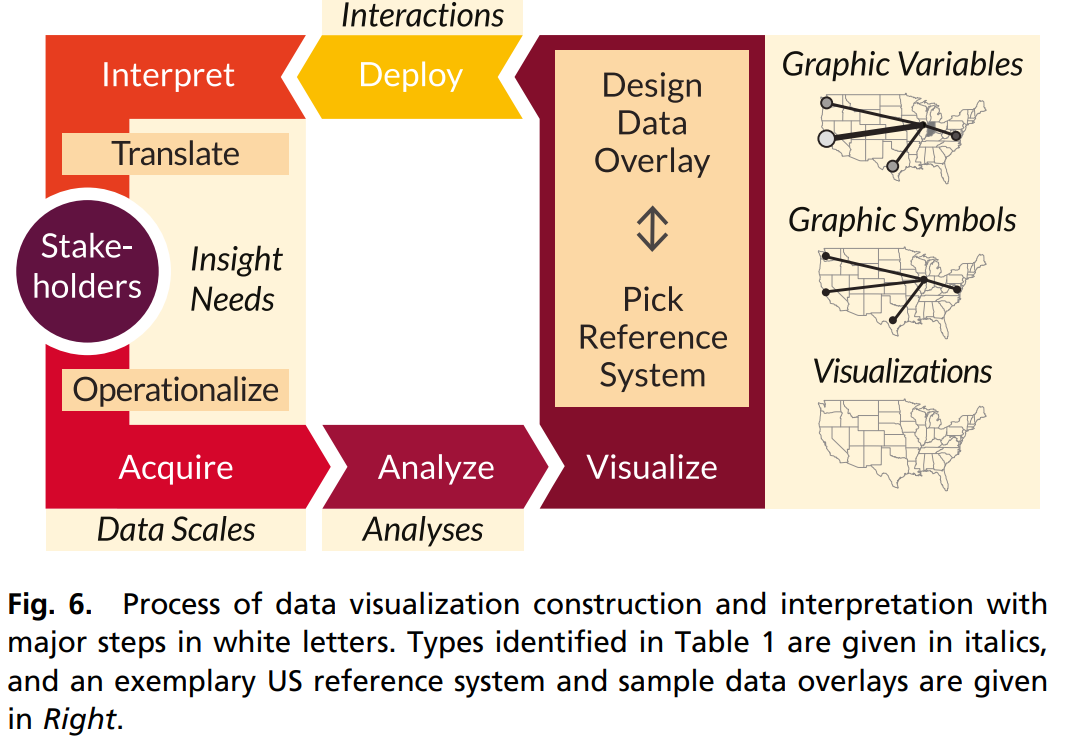
\includegraphics[width=.9\linewidth]{images/borner2019_figure6.png}
	\caption{Process of data visualization construction and interpretation with major steps in white letters. Types identified in Table 1 are given in italics, and an exemplary US reference system and sample data overlays are given in Right. (Borner2019)}
	\label{fig:borner2019_fig6}
\end{figure}

\subsubsection{Data manipuliation}
-{\color{orange}Geoportals can also offer online processing functionalities, ranging from basic transformations (e.g. coordinate reference system re-projection, sub-setting, format mapping) to complex algorithms for classification, and statistical analysis. That may require an underlying infrastructure providing a workflow engine to orchestrate the multiple actions required to implement the required processing.”\cite{Jiang2020}}\\
-{\color{orange}Spatial queries require indices (such as R-trees or quadtrees) for efficient execution.\cite{Lieberman2010}}\\
-{\color{orange}Zoom: “smooth zooming helps users preserve their sense of position and context”.\cite{Shneiderman1996}}\\
-{\color{orange}Filter: “By allowing users to control the contents of the display, users can quickly focus on their interests by eliminating unwanted items.''\cite{Shneiderman1996}}\\
-{\color{orange}History: “It is rare that a single user action produces the desired outcome. Information exploration is inherently a process with many steps, so keeping the history of actions and allowing users to retrace their steps is important.”\cite{Shneiderman1996}}\\
-{\color{orange}“Dynamic queries can reveal global properties as well as assist users in answering specific questions.”\cite{Shneiderman1996}}\\
-{\color{orange}“dynamic visualizations: overview, zoom, filter, details on demand, relate (viewing relationships among items), history (keeping a log of actions to support undo, replay, and progressive refinement), and extract (access subcollections and query parameters)”\cite{Borner2019}}\\
-{\color{orange}“Keim distinguishes zoom filter, and link and brush as well as projection and distortion techniques as a means to provide focus and context.”\cite{Borner2019}}\\
-{\color{orange}“Brehmer and Munzner covers two main abstract visualization tasks. The first is ‘why’, which includes consume (present, discover, enjoy, produce, search (lookup, browse, locate, explore), and query (identify, compare, summarize). The second is ‘how,’ which consists of encode, manipulate (select, navigate, arrange, change, filter, aggregate), and introduce (annotate, import, derive, record).”\cite{Borner2019}}\\
-{\color{orange}Other setup: “data and view specification (visualize, filter, sort, derive), view manipulation (select, manage, coordinate, organize), and process and provenance (record, annotate, share, guide).”\cite{Borner2019}}\\

\subsubsection{Security}
-{\color{orange}“some people might be concerned about sharing their identify in online environment or making their profile information visible, as they are worried about organizational and social threats”.}\cite{Afzalan2017}.\\
-{\color{orange}“For implementing these common functionalities, additional functionalities are often required. For example, a geoportal should implement a subset of functionalities concerning privacy and security aspects, e.g. authentication, data access control, logging. Moreover, the geoportal administrators need dedicated management functionalities. \cite{Jiang2020}}\\


\subsubsection{Products}
-{\color{orange}Recommended services for geoportals: catalogue, preview, access, and online analysis and processing \cite{Jiang2020}}\\
\textbf{RSS}\\
-{\color{orange}“Publish/Subscribe has emerged as a communication paradigm able to facilitate the development of complex distributed applications in open network environments. THe strong decoupling it introduces between communication parties enables applications to publish information without being aware of the identities of potential receivers or even of their existence.  Similarly, it enables receivers to issue subscriptions that express their interests in messages with a given content regardless of the identity of their publishers.”}\cite{Xing2015}\\
-{\color{orange} “GeoRSS is an emerging standard for RSS feeds to be descried b location or geo-tagged in a standardized way in which the location is encoded. Many map APIs support GeoRSS feeds with either coordinate (lat/long) data or address information specified in XML items. “}\cite{Xing2015}\\
-{\color{orange} Geoportal design: Download tool: ``A download tool incorporates the capability of obtaining data and metadata. Metadata could be downloaded by XML structured files, and data could be downloaded as raster or bector based data outputs through various ways, such as FTP'' \cite{Jiang2020}}\\
-{\color{orange} GeoRSS feed suppor \cite{Marshall2012}}\\

\textbf{API}\\
-{\color{orange}“it is suggested to provide tools (e.g. API, widgets, configuration) to create community portals, and applications tailored to specific users. THey would allow developing, discovering, and running of applications to support different online and cloud based scenarios in particular for big earth data processing… Geoportals could involve online spatial analysis functionality for addressing geospatial analysis tasks, e.g. online computing environments and geospatial processing web, online analysis, and cloud computing.”\cite{Jiang2020}}\\
-{\color{orange}“Geoportals could also provide APIs to enable developers to create alternative user interfaces to data systems, including community portals and mobile/desktop apps.” Incorporate API functionality.\cite{Jiang2020}}\\
-{\color{orange}“System components communicate using open application programming interfaces (APIs) so that each component can be replaced by a different technology if necessary.” GeoAnnotator \cite{Karimzadeh2019}}\\

\subsubsection{Dashboard design}
-{\color{orange}“Viewing multiple folded and aligned units of event sequences simultaneously and in their entirety would require considerable screen space. However, aggregation can obscure rapid changes and outliers. Overview and detailed approaches are beneficial in these cases.”\cite{Zhang2019}}\\
-{\color{orange}“The benefit of superimposing time series from multiple days is to allow direct comparison without changing the view. However, these line charts may cause significant visual clutter and conflicts. Superimposing distinct views can sidestep this problem.\cite{Zhang2019}}\\
-{\color{orange}“Our participants appreciated and were able to effectively use superimposed distinct visualizations of multivariate data in the overview and detail panels.”\cite{Zhang2019}}\\

\subsubsection{Internationalization and localization}
%See links from wikipedia: https://en.wikipedia.org/wiki/Internationalization_and_localization#cite_note-SFW-1
%“split each potentially locale-dependent part (whether code, text or data) into a separate module. Each module can then either rely on a standard library/dependency or be independently replaced as needed for each locale.” wikipedia
%“place text in resource strings which are loaded during program execution as needed.”
-{\color{orange}“Localization refers to the adaptation of a product application or document content to meet the language, cultural and other requirements of a specific target market (a ‘locale’).\cite{Ishida2005}}\\
-{\color{orange} Localization: l10n \cite{Ishida2005}}\\
-{\color{orange} “Internationalization is the design and development of a product, application or document content that enables easy localization for target audiences that vary in culture, region, or language.”\cite{Ishida2005}}\\
-{\color{orange} Internationalization: i18n\cite{Ishida2005}}\\
-{\color{orange} “Retrofitting a linguistically- and culturally-centered deliverable for a global market is obviously much more difficult and time-consuming than designing a deliverable with the intent of presenting it globally.”\cite{Ishida2005}}\\
-{\color{orange} “So ideally, internationalization occurs as a fundamental step in the design and development process, rather than as an afterthought that can often involve awkward and expensive re-engineering.”\cite{Ishida2005}}\\
%{\color{orange}Localization customization: “1. Numeric, data and time formats 2. Use of currency 3. Keyboard usage 4. Collation and sorting 5. Symbols, icons and colors 6. Text and graphics containing references to objects, actions or ideas which, in a given culture, may be subject to misinterpretation or viewed as insensitive. 7. Varying legal requirements 8. and many more things.”\cite{Ishida2005}}\\
%{\color{orange} Internalization: “1. Designing and developing in a way that removes barriers to localization of international deployment. This includes such things as enabling the use of unicode, or ensuring the proper handling of legacy character encodings where appropriate, taking care over the concatenation of strings, avoiding dependency in code of user-interface string values, etc. 2. Providing support for features that may not be used until localization occurs. FOr example, adding markup in your DTD to support bidirectional text, or for identifying language. Or adding to CSS support for vertical text or other non.-Latin typographic features. 3. Enabling code to support local, regional, language, or culturally related preferences. Typically this involves incorporating predefined localization data and features derived from existing libraries or user preferences. Examples include date and time formats, local calendars, number formats and numeral systems, sorting and presentation of lists, handling of personal names and forms of address, etc. 4. Separating localizable elements from source code or content, such that localized alternatives can be loaded or selected based on the user’s international preferences as needed.”\cite{Ishida2005}}\\



\subsubsection{Examples}
\textbf{Geo my WordPress}\\
-{\color{orange}“Geotag any of your post types, buddypress members and other components”\cite{Fitoussi}}\\
-{\color{orange}“Create unlimited advanced, proximity search forms to search and find any of the geotagged components of your site”\cite{Fitoussi}}\\
-{\color{orange}“Add geographic location to any of the registered post types of your site. Display post location on a map, and create proximity search forms to search and find posts based on address, distance categories and more.”\cite{Fitoussi}}
%-{\color{orange}“Create unlimited mashup maps and proximity search forms to search and find post types, BuddyPress members, and other components, based on an address, distance, categories, profile fields, and more.”\cite{Fitoussi}}\\
-{\color{orange} Based on Google Maps API, also supports Leaflet and OpenStreetMaps\cite{Fitoussi}}\\
-{\color{orange} Reviews: 4.6/5 stars.\cite{Fitoussi}}\\
-{\color{purple} Appears to only be for point data (not area)\cite{Fitoussi}}\\

\textbf{NewsPack}\\
-{\color{orange} A wordpress model for news sources (mostly american) \cite{Carvalho2020}}\\\
-{\color{orange} The backoffice 60\% of global news rooms \cite{Carvalho2020}}\\
-{\color{orange} Doesnt' allow for customization \cite{Carvalho2020}}{\color{purple} Opportunity to create a plugin for wordpress to accomplish this}
-{\color{orange} Easy to work in\cite{Carvalho2020}}\\
-{\color{orange} Mostly tailored to US local news \cite{Carvalho2020}}\\
-{\color{purple} Doesn't incorporate or recommend a geolocation element \cite{newspack}}\\

